\documentclass[DM,lsstdraft,toc]{lsstdoc}
\usepackage{graphicx}
\usepackage{url}
\usepackage{latexsym}
\usepackage{color}
% black, blue, brown, cyan, darkgray, gray, green, lightgray, lime, magenta, blue, orange, pink, purple, red, teal, violet, white, yellow.
\usepackage{enumitem}

\title[LSST Special Programs]{Data Management \\ and LSST Special Programs}

\author{M.~L.~Graham, M.~Juri\'{c}, K.-T.~Lim, and E.~Bellm}

\setDocRef{DMTN-065}
\date{\today}
\setDocRevision{TBD}
\setDocStatus{draft}

\setDocAbstract{\textbf{This is a draft document and may yet change.} The purpose of this study is to ensure that the LSST Data Management's plans for processing data from Special Programs (Deep Drilling Fields and Mini-Surveys) will meet the needs of the scientific community, and that these plans have been appropriately sized for computational processing and are accurately represented in the work-hours budget. Unresolved issues spawn \textbf{Actions}, which are typically documentation change requests or proposed studies to assess a potential problem.}

\setDocChangeRecord{%
\addtohist{1}{2017-11-??}{Internal working document.}{Melissa Graham}
%\addtohist{2}{yyyy-mm-dd}{Future changes}{Future person}
}

\begin{document}

\maketitle

% CITATION EXAMPLES
% \verb|\citellp|: \citellp{LPM-17, LSE-30} \\
% \verb|\citell|: (SRD; \citell{LPM-17,LSE-29}) \\
% \verb|\citep[][]|: \citep[e.g.,][are interesting]{LPM-17,LSE-29} \\
% \verb|\cite|: \cite{LPM-17,LSE-29}



% % % % % % % % % % % % % % % % % % % % % % % % % % % % % % % % % % % %
\section{Introduction} \label{sec:intro}

The intent of the LSST Data Management team for processing data from Special Programs can be summarized by the following statement, which reflects Section 6 of the Data Products Definitions Document (\DPDD, \citeds{LSE-163}; but see also the minor proposed change to this statement in \ref{Size-1}):

\begin{quote}
LSST will not write unique algorithms for processing Special Programs data or reprocessing Main Survey data, but LSST will reconfigure the pipelines and generate imaging and catalog products for Special Programs data whenever possible, and LSST will make its codes accessible to the science community and commit $\sim$10\% of its computing resources toward enabling Level 3 analysis and data product creation, including user-driven Special Programs processing.
\end{quote}

\noindent The purpose of this study is to ensure that the requirements and plans of DM are accurately expressed in all major DM documentation, and that the computational system and human work-hours needed to accomplish Special Programs processing have been accurately evaluated. This study spawns \textbf{Action} items, which are typically either documentation change requests or proposals for future studies needed to resolve an issue.

%In particular, this study is designed to review: (1) the processing and products that are required to enable science for Special Programs, (2) the current plans for DM processing and products with respect to Special Programs, (3) whether the DM plans meet the expected needs of Special Programs, and (4) any necessary changes to be written into the requirements, designs, and plans, in which case an \textbf{Action} is spawned.

Section \ref{sec:data} compiles an overview of the potential diversity in data from Special Programs, compared to the Wide-Fast-Deep (WFD) main survey data: standard visit images of $2\times15$ seconds for a wide area of the nighttime sky, obtained with a dither pattern using up to five filters. We assemble the possible limitations on Special Programs observations from the capabilities of the telescope and camera.

Section \ref{sec:dmplans} reviews the current DM plans for processing Special Programs data, including the capabilities for processing non-standard visits and whether DM might need to impose boundaries on the parameters of non-standard images that its pipelines will be able to processes. We also describe DM's intent for incorporating Special Programs data into the WFD main survey products, reconfiguring pipelines to create unique products, and providing support for end-user Level 3 processing.

Section \ref{sec:docrev} steps through each of the relevant LSST documents and highlights specific requirements or text in these documents that might need additions or clarifications to properly reflect DM's plans for processing Special Programs data.
%These \textbf{Concerns} are not prioritized by urgency or importance, but instead represent more of a complete set of possible issues. \textbf{The Concerns raised by this study fall into two main categories:} \\
%1. Whether DM will be able to process the full diversity of non-standard visit images, and if not, what the boundaries will be. \\
%2. Ensuring that DM's intent to process Special Programs data with reconfigured pipelines, and to provide separate data products that meet the science goals of each program, is accurately reflected in all documents, as it is in the DPDD, and is in the staffing budget. \\

Section \ref{sec:SP_SC} gathers the existing efforts from the Science Community regarding Special Programs, summarizes the scientific needs of as many currently proposed Special Programs as we can find, and outlines the future mechanisms for LSST to gather more community input -- including some recommendations for the future call for Special Programs white paper proposals.

Section \ref{sec:SPCS} contains a series of case studies for DM's processing of Special Programs data, which are based on several of the currently circulating ideas for deep drilling fields and mini-surveys. These processing case studies contribute to this work by offering an independent vantage point from which to identify a few additional issues regarding the processing of Special Programs data, and could also serve as examples for the upcoming call for community white papers, which will request that a similar section be included in all proposals.


% % % % % % % % % % % % % % % % % % % % % % % % % % % % % % % % % % % %
\clearpage
\section{The Potential Diversity of Special Programs Data} \label{sec:data}

To better identify what might be missing in the DM plan to accommodate Special Programs, we need a comprehensive understanding of the potential diversity in future Special Programs data. The concern is that if Special Programs data is significantly different from the Wide-Fast-Deep survey of tiled, nighttime, 15--30 second exposures (i.e., standard visit images), then it might not be adequately handled by the DM system. To get an idea of the potential diversity of Special Programs data, we first attempt to understand the technical limitations that the facility and instrumentation places on the observing modes, e.g., exposure times, filter changes, in Section \ref{ssec:data_bounds}.

We can also get an idea of the expected diversity in exposure type and survey pattern from the current set of proposed Special Programs for LSST, which are reviewed in more detail in Section \ref{sec:SP_SC}. We find that most of the proposed Special Programs are likely to use standard visits, two $\sim15$ second exposures, and that the potential diversity of Special Programs data is mainly comprised of exposures that are significantly shorter than the WFD main survey standard visit exposures of $2\times15$ seconds, exposures that are obtained with a bright sky background during twilight, long series of exposures obtained of the same field (i.e., deep drilling), and images of crowded fields.

All aspects related to DM's \textit{processing} of Special Programs data are addressed in Section \ref{sec:dmplans}.

% % % % % % % % % % % % % % % % % %
\subsection{Technical Boundaries for Special Programs Data}\label{ssec:data_bounds}

We can constrain the potential diversity of Special Programs data if we know the observing boundaries that will be imposed on the accepted proposals. For the purposes of this document we consider the ``observing boundaries" as those imposed by the camera, telescope, or site, and independent of any DM processing capabilities. It is not the job of this document to define these observing boundaries, but we do need to know what they are in order to predict the diversity of incoming data that DM will be processing.

The current technical limitations on what kind of observations can be obtained with the LSST telescope and camera are described below in a rough draft, to be updated in the future. Additionally, in Section \ref{ssec:docrev_oss}, we review the Observatory System Specifications (OSS, \citeds{LSE-30}) document and highlight a couple more questions regarding potential boundaries on Special Programs observations.

Filter Changes: \\
$\bullet$ The maximum time for filter change is 120 seconds: 30 seconds for the telescope to reorient the camera to its nominal zero angle position on the rotator, and 90 seconds to the camera subsystem for executing the change (OSS-REQ-0293). \\
$\bullet$ Note that changes regarding the requirements on filters in support of "deep drilling fields" are underway here: \href{https://project.lsst.org/groups/ccb/node/938}{LCR-458}. \\
$\bullet$ \textit{(MLG - The next three points are from a document-in-progress by Ivezic and Ritz; update to formal citation when it's public-facing.)} \\
$\bullet$ The minimum time between filter changes has no restrictions from e.g., thermal tolerances. However, based on overheads and efficiency, it is recommended to keep the filter change rate lower than once every 10 minutes. \\
$\bullet$ The maximum total number of filter changes is 100,000 over 15 years, an average of 18 changes per night. \\
$\bullet$ The maximum number of filter swaps in/out of the carousel is 3000 in 15 years, or once every two nights. \\

Exposure Times: \\
$\bullet$ The minimum exposure time is 1 second, with a stretch goal of 0.1 seconds (OSS-REQ-0291). \\
$\bullet$ The maximum exposure time is not restricted. \\
$\bullet$ However, for exposure times there are other considerations. The minimum exposure time needed to create an image with a PSF that is well-formed enough for difference imaging is a separate question. Changing the exposure time also affects the photometric and astrometric calibrations. Assuming a 1 second exposure can be reduced and calibrated, its detected point sources will span $13 < r < 21$ magnitudes, whereas a 15 second exposure saturates at $r\sim15.8$ mag. A 150 second image would saturate at $r\sim18.3$, perhaps leaving too few stars overlapping with e.g., templates or WFD images, for astrometric and photometric calibrations. Additionally, the impact on CR rejection routines is untested for long exposures.

Camera Rotation: \\
$\bullet$ The OSS contains requirements for rotator capability (OSS-REQ-0301, -0300), but is there a maximum rotation speed, or a limit on the amount of rotation per night (or in a 10-year lifetime), that might constrain the distance between successive visits or the ability to jump between two widely separated fields? \textit{MLG - I heard there might be a lifetime maximum on the rotator, such that if a mini-survey wants to jump between patches that are far apart on the sky repeatedly, that could wear out the mechanism? Can't remember where I heard it.}

Telescope Slews: \\
$\bullet$ \textit{MLG - Obviously, long slews would cause additional overheads and a loss of observing efficiency, but are there other limitations?}

Total Time: \\
$\bullet$ It has been regularly stated that 10\% of the total observing time will be used for special programs (90\% goes to the WFD main survey). This could be increased a bit, but otherwise imposes an upper limit on the total time request of a given Special Program.

Operations Simulations: \\
$\bullet$ Mini-survey observing strategies will have to show that they do not negatively impact the LSST's ability to complete the wide-fast-deep survey; not necessarily in the next call for white papers, but later during the review and revise stage, once the new OpSim runs incorporating proposed mini-surveys have been generated.

\begin{enumerate}[resume,topsep=-10pt,after=\vspace{10pt},label= \textbf{Action \Roman*}] \item \label{Bounds-1} The purpose of this ticket is to request clarification regarding several aspects of the telescope and camera capabilities that might impose boundaries on the diversity of data from Special Programs. First, have the following proposed filter change tolerances been confirmed: (1) the minimum time between filter changes has no restrictions from thermal tolerances, but it is recommended to keep the filter change rate lower than once every 10 minutes in order to minimize overheads; (2) the maximum total number of filter changes is 100000 over 15 years (18/night) and the maximum number of filter swaps in and out of the carousel is 3000 in 15 years (once every two nights). Second, are there any restrictions on the use of the camera rotator or the total amount of slew time? For example, could a Special Program continuously jump between well-separated fields on the sky for an extended amount of time? \end{enumerate}


% % % % % % % % % % % % % % % % % % % % % % % % % % % % % % % % % % % %
\clearpage
\section{The Current DM Plans for Special Programs Data Processing} \label{sec:dmplans}

As presented in Section \ref{sec:intro}, the intent of LSST DM for processing data from Special Programs is that ``LSST will not write unique algorithms for processing Special Programs data or reprocessing Main Survey data, but LSST will reconfigure the pipelines and generate imaging and catalog products for Special Programs data whenever possible" (\DPDD, \citeds{LSE-163}), and that an additional $\sim$10\% of the LSST computational system has been added and will be dedicated to user processing (of main survey or special programs data).

In this section we review in greater detail the planned ability of DM to process non-standard visit images (Section \ref{ssec:dmplans_NSV}), the intent of DM to incorporate Special Programs data into the pipelines and products for the WFD main survey (Section \ref{ssec:dmplans_WFD}), to reconfigure the pipelines and generate unique sets of data products for each Special Program (Section \ref{ssec:dmplans_reconfig}), and to enable Level 3 processing (Section \ref{ssec:dmplans_L3}).

% % % % % % % % % % % % % % % % % %
\subsection{DM Constraints on Processing Non-Standard Visit Images}\label{ssec:dmplans_NSV}

A standard visit image is considered to be two snap exposures of $\sim15$ second each, and in the WFD main survey sequential visits will be of different fields. As we found in Section \ref{sec:data}, Special Programs are most likely to request observing modes with shorter exposure times and long sequences of visits to the same field. In this section we review DM's planned capability to process such non-standard visit sequences, keeping in mind that DM's processing boundaries might ultimately be defined not by exposure acquisition parameters, but by the image quality parameters such as number of stars with sufficient flux for calibration or the source area density (crowding), and that these boundaries might not be fully constrained until the final performance of DM algorithms as described in the Data Management Applications Design (DMAD, \citeds{LDM-151}) document are characterized (see also Section \ref{ssec:docrev_dmad}).

\subsubsection{Exposure Times}

Images which deviate significantly from the $15$ second duration for the WFD main survey may encounter issues in the instrument signature removal routine, in difference imaging and the correction for differential chromatic refraction, and/or photometric and astrometric calibrations due to a differently sampled set of standard stars per CCD. We consider shorter and longer exposure in turn.

\textbf{Shorter Exposures.} The camera constraint on the minimum supported exposure time is currently 1 second (stretch goal 0.1 seconds). The minimum exposure time for an image to be successfully reduced with Instrument Signature Removal (ISR) will be a DM constraint. Assuming that 1 second exposure can be reduced and calibrated, its detected point sources will span a dynamic range of $r \approx 12.9$ -- $21.0$ magnitudes. A template image built on $15$ second exposures will saturate at $r \approx 15.8$, but this still leaves stars between $15.8$--$21.0$ magnitudes to be used in the PSF-matching (and all other filters have a similarly large overlap). However, in order for an image to be successfully PSF-matched to the template, the PSF must be well formed (i.e., no speckle pattern), and have a spatial variance that the pipeline is capable of modeling (i.e., be smoothly varying on some minimal scale). As a simple demonstration, MLG has made Figure \ref{fig:expt} to show that perhaps exposure times shorter than 2 seconds do not have a well-formed PSF (using the centroid of a 2D Gaussian fit as a proxy for "well-formed"). Another concern is that the Level 1 pipeline would not be able to deliver the required $60$ second latency if the camera produces more than 1 image in 30 seconds, which would disqualify a contribution to the Alert Stream.

\begin{figure}
\begin{center}
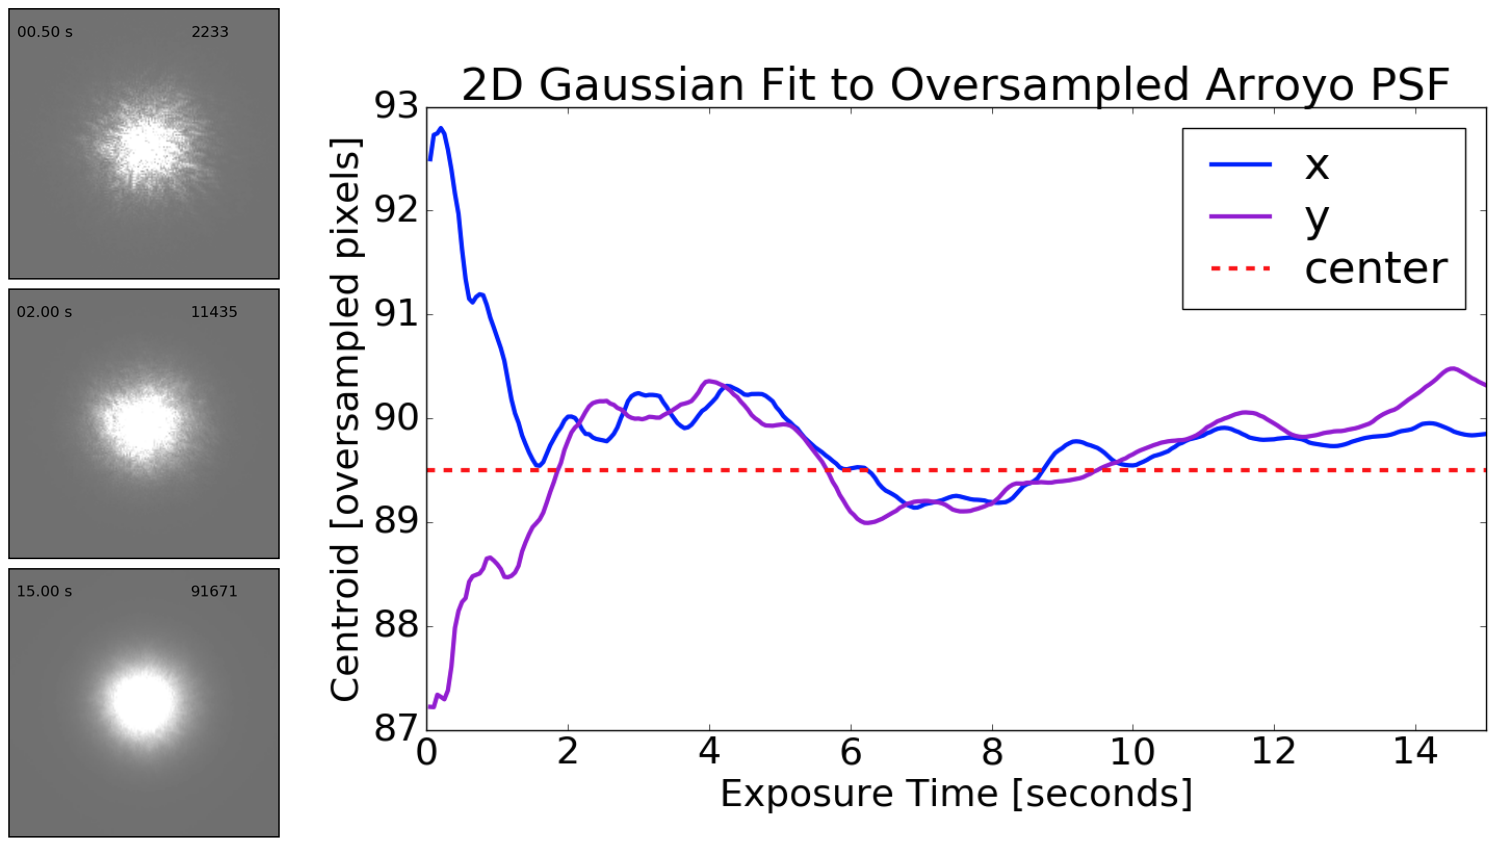
\includegraphics[width=14cm,trim={0cm 0cm 0cm 0cm}, clip]{figures/exptime.png}
\caption{At left, Arroyo atmosphere-only simulated PSF for LSST (with oversampled pixels) with exposure times of 0.5, 2, and 15 seconds (top to bottom), courtesy of Bo Xin. At right, blue and purple lines show the location of the centroid derived from a 2D Gaussian fit to the PSF as a function of exposure time, with the red dashed line showing the true center. We can see that for exposure times greater than 2 seconds, the centroid converges near its true value. \label{fig:expt}}
\end{center}
\end{figure}

\textbf{Longer Exposures.} There is no maximum exposure time specified for an LSST image. Given that the template image will be a stack of at least a year or two of data, processing a $5$--$10$ times deeper single image through the difference imaging pipeline should be fine. However, a $2\times150$ second exposure would saturate at $r \approx 18.3$, and cosmic-ray rejection completeness might suffer (unknown), which could impact the quality of a difference image and the detected sources. With a longer exposure time the $60$ second latency requirement could still be met, but any system qualities that vary on short (but $>30$ second) timescales could inhibit photometric calibration (e.g., tracking).

In conversation with DM-AP team members (Reiss, Findeisen, Connolly, Bo) there has not yet been a study of the safe range of exposure times that will be allowed to contribute to the Level 1 and Alert Stream. One possibly useful study is Chang et al. (2012), "Atmospheric point spread function interpolation for weak lensing in short exposure imaging data". They show that a 15 second exposure contains PSF variability on short spatial scales across a 1 square degree image which, for extragalactic fields with few stars (i.e., but good for weak lensing), is hard to characterize. They present a new software package to do mitigate the effects. Alternatively, we may need to use software packages \texttt{PhoSim} (Peterson et al. 2015; \url{http://adsabs.harvard.edu/abs/2015ApJS..218...14P}) or \texttt{ARROYO} (\url{http://proceedings.spiedigitallibrary.org/proceeding.aspx?articleid=848256}) to at least simply characterize the PSF stability as a function of exposure time.

In conversation with K.-T., exposure times of 10 to 120 seconds will not be a problem for the processing pipeline to accommodate, but the ingest rate of images and the number of exposure per visit are the aspects that could cause issues (discussed below).

Is it conceivable that the LSST would spend time on a Special Program that will acquire short exposures if DM's algorithms cannot be shown to adequately reduce and calibrate them? This is probably best left ot a policy issue (beyond the scope of this document).


\subsubsection{Image Acquisition Rate}

OSS-REQ-0291 requires that short exposures be spaced by 15 seconds, and so DM's ingest rate of exposures should never be more than 1 per 15 seconds, or a visit rate of 1 per 30 seconds. However, \textit{if a higher image acquisition rate is cleared by the camera team}, then DM might encounter some issues such as the minimum time required to save an image to disk, the handling of a processing backup, and/or inconsistently associated \texttt{DIASources}.

\textbf{Minimum Save Time:} If short exposures are taken in an unbuffered sequence, the minimum time between exposures is the shutter-crossing time (1 second) plus the readout time (2 seconds): 3 seconds. This is too rapid an acquisition rate for processing with Level 1, but what if the science goals accept saving them to disk and analyzing them later? \textbf{How long does it take to save an image to disk?}

\textbf{Processing backup:} Are there options for short-term increases in parallel processing power at NCSA? (Such options might be needed anyway to process crowded fields with $>$10k \texttt{DIASources}.) The bandwidth needed to load templates at a faster rate is also a concern, since templates have twice as many pixels, if the data acquistion rate is surveying at twice the WFD main survey rate, that's a $4\times$ additional bandwidth load. However, at NCSA there should be ways to elastically change the amount of processing power available. This is also an issue for crowded fields (below).

\textbf{Unassociated \texttt{DIASources}:} the consistency of \texttt{DIAObjects} suffers if the same patch of sky is observed in quick succession (overlapping regions of short exposures and/or sustained 30 second visits to the same field). In other words, it is not guaranteed that the next string of processing would have access to the latest \texttt{DIAObjects} for association. It is furthermore unclear whether we can flag an Alert as potentially having incomplete source-object associations. This is also an issue for crowded fields (below).

\subsubsection{Exposures per Visit, and Long Sequences of a Single Field}

K.-T. Lim has pointed out that an odd number of exposures is a non-standard visit; two snaps is hardwired into the code. This is baked-in to a configuration so that the pipeline can have a definition of what kind of timing delay constitutes ``late".  Moving away from 2 exposures per visit requires a configuration change to the pipelines, which incurs an overhead (up to 1 minute) -- in fact, K.-T. things that between $10$ and $120$ seconds exposure times can easily be handled by the pipeline (i.e., can be run through ISR using scaled calibration frames), so long as they come in pairs. The real problem is knowing how long the processing should take, and not killing a process that is taking longer because there were 4 snaps in the visit instead of 2. To accommodate non-standard visits requires that the scheduler pass on the information of the number of snaps in the visit (\ref{DMSR-1}). Then the processing pipeline will know to, e.g., not attempt to difference the two snaps in the case were there is an odd number of snaps in a visit. \textit{MLG -- I've heard rumors of a CR regarding alternate standard visits of $1\times30$ seconds, but do not know the status or implications of this.}

K.-T. has also pointed out that currently, a deep drilling field would be interpreted as a single visit of 50 exposures by the scheduler. One implication of this is that since the camera only ``clears" prior to a new visit, it would not do this for the entire 50-exposure sequence. The processing pipeline would need to know how to divide this sequence up into visits. As there is no current requirement for DM to receive the information that the scheduler is about to do a 50 exposure visit, we need \ref{DMSR-1} to add the proposal ID and the number of exposures per visit to the meta data, and then it should be OK for DM to parse this visit information in the reduction pipeline.

\subsubsection{Alerts from Crowded Fields}

Special Programs are more likely to include crowded fields than the WFD main survey area. Due to the increased number of sources, the number of \texttt{DIASources} -- and therefore the number of Alerts -- increases as well. In turn, this increases the processing time and in some cases, may exceed the 60 second limit for Alert Production. A policy is needed on whether Alerts from crowded fields should be allowed a delay, or allowed to be incomplete. K.-T. reports that the control system can easily kill processes that are running over time and move forward with existing outputs -- but that perhaps it will be just as easy to let it keep running and elastically grab additional NCSA resources as needed. This appears possible because the batch system is larger than the Level 1 allocation, although we might not know that this is possible until Level 1 integration happens at NCSA (see Document LDM-230, the operations concepts).

\subsubsection{Summary}

\begin{enumerate}[resume,topsep=-10pt,after=\vspace{10pt},label= \textbf{Action \Roman*}] \item \label{NSV-1} The purpose of this ticket is to ensure that DM's capability for processing non-standard visit images, and required by LSR-REQ-0111, will meet the needs of Special Programs data (which might be considerably more diverse than data for the wide-fast-deep main survey). For now we have adopted a broad interpretation of ``processing" to mean both the initial ISR stage and also the Level 1 Alert Production pipeline, because allowing as many LSST images as possible to contribute to the Alert Stream is a benefit to time domain science. After comparing the anticipated potential diversity in Special Programs data with the currently planned DM pipelines, we have identified several open questions that need to be resolved in advance of the call for Special Programs white papers in the spring of 2018. (1) What is the anticipated minimum (and maximum, if applicable) exposure time for an image to be successfully processed by ISR and DIA? In the latter case, this will probably be limited by the time needed to generate a well-formed PSF. (2) Presently, OSS-REQ-0291 requires that even short exposures be spaced by 15 seconds. Might this requirement be slackened to accommodate a higher cadence Special Program? If so, and if Level 1 processing is required for the science goals, then DM will need to assess options to elastically increase NCSA computational resources and/or the policy for dropping \textit{vs.} delaying Alerts during observations with a fast ingest cadence. These issues apply also to Special Programs in the Galactic plane, where crowded fields will increase the volume of Alerts. Alternatively, we could formally require that only 30 second visits will be allowed to contribute to Level 1 Alert Production (3) Long sequences of images on a single field are a likely Special Programs mode (e.g., DDF). We need to confirm that the processing pipeline has the ability to re-parse a scheduled $N$-exposure visit into standard $2$-exposure visits. Consequential images of the same field may lead to unassociated \texttt{DIASources} of the same \texttt{DIAObject}, and it should be confirmed that the DM pipelines can recognize this when it happens, and flag the resulting Alerts appropriately. \end{enumerate}


% % % % % % % % % % % % % % % % % %
\subsection{Intent to Include Special Programs Data in the WFD Survey Products}\label{ssec:dmplans_WFD}

DM will want to incorporate images obtained through Special Programs into the WFD main survey's pipelines and products whenever it is beneficial for enabling science. In the following three sections we summarize when and how Special Programs data might be incorporated into the pipelines and products of the Difference Imaging Analysis and Alert Stream, the Data Release Pipeline products, and/or MOPS.

\subsubsection{Level 1 and the Alert Stream}\label{ssec:dmplans_WFD_L1}

It is beneficial to transient science to include as many LSST images into the Level 1 Difference Imaging Analysis and Alert Stream as possible. Only products of the Level 1 $60$-second processing pipeline can contribute to the Alert Stream: this means that no Level 3 difference imaging pipeline can send its detections to the Alert Stream, although a separate Level 3 alert stream should be possible if the packet/transport mechanism that LSST defines is adopted outside of LSST (this prospect is discussed further in Section \ref{ssec:dmplans_L3}). Therefore, only images that qualify for Level 1 processing will contribute to the Alert Stream. DM's ability to process the potential diversity of image types from Special Programs is explored above in Section \ref{ssec:dmplans_NSV}, and we continue the discussion of incorporating processed images into the Level 1 DIA pipeline.

\textbf{Templates:} The template images that are used in the Level 1 difference imaging pipeline will be built from the Level 2 DRP, and so the first factor affecting a Special Programs image's suitability for Level 1 is to be in a region of sky with an existing template. So long as there is a template, when the exposure time is equivalent to a WFD visit image, $\sim 30$ seconds, treating the image as Level 1 is going to be fine. When processing Special Programs data with the Level 1 pipeline, certain science cases might call for the capability to load and use a certain template that is different from the WFD template (i.e., built over a different timescale). K.-T. confirms that there is not enough memory allotted to store more than one template over the whole sky, but for sub-regions, storing and using an alternative template should be possible. This is not an issue limited to Special Programs, since during commissioning it is conceivable that multiple template versions. K.-T. also confirms that the capability for the processing pipeline to choose a given template based on the programID in the raw image metadata will exist.

\subsubsection{MOPS}\label{ssec:dmplans_WFD_MOPS}

The WFD main survey observations will be optimized to meet the mandated goals for moving object discoveries, so it is unclear whether the science goals of MOPS can be much improved by incorporating Special Programs data (aside from e.g., the North Ecliptic Spur area, which has been treated as a Mini-Survey region that will generate a larger number of SSO discoveries). Since MOPS takes \texttt{DIASources} as input, any Special Programs images that can be run through the Alert Pipeline can be ingested by MOPS. As discussed under "Solar System Objects (SSO)" in Section \ref{ssec:data_science}, most of the Special Programs data associated with SSO science will obtain standard visit images anyway. There was some concern that a large number of small-separation sources might overwhelm the processing system (i.e., from a deep drilling field with many exposures in a sequence), but upon further consideration this worry was rejected.

\subsubsection{Level 2 Data Release Pipeline}\label{ssec:dmplans_WFD_L2}

Unlike with transient detection and the Level 1 Alert Stream, it is not clear whether it is beneficial to the science goals that depend on the Level 2 DRP to include as many LSST images as possible. We propose that the simplest option is probably that LSST DM deliver a single Level 2 DRP \texttt{Objects} database that is built from a set of images with nearly constant depth and cadence. When Special Programs data brings additional area up to the same level of depth and cadence as the rest of the WFD main survey, or improves the Level 2 DRP in some other way, it can be included in the Level 2 DRP. For example, photometric calibrations may require that some or all of the (shallower) Galactic Plane Special Program survey area be incorporated in order to suppress edge effects and low-order modes in the photometric solutions. In short, DM should probably not promise to incorporate any specific data into the Level 2 DRP images or catalogs, and it will not be the default to include Special Programs data into the products for the WFD main survey. This is mostly discussed here in context with the \texttt{Source} and \texttt{Object} catalogs and the deep CoAdds, but also applies to the DIA pipeline products.

% % % % % % % % % % % % % % % % % %
\subsection{Intent to Process Special Programs Data with Reconfigured DM Pipelines}\label{ssec:dmplans_reconfig}

LSST DM intends to reconfigure its existing pipelines in order to generate unique and separate -- but joinable -- imaging and catalog products for Special Programs data, whenever possible. In this context, ``possible" means that no new algorithms need to be written and that an intensive amount of additional computational resources is not required for the processing.

In a ``possible" scenario, DM would assemble a pipeline from existing DM codes in order to process data associated with a given Special Program and build image and catalog products that meet the science needs of that particular program. For example, for a DDF SN survey (see Section \ref{ssec:SPCS_SNDDF}), existing DM codes would be used to: (1) make a deep template image from a certain time window, (2) process standard single visit images, (3) create a nightly CoAdd, (4) run difference imaging analysis, (5) run source detection on the difference images, and (6) create \texttt{DIASource} and \texttt{DIAObject} catalog equivalents (this example is also given in Section 6 of the \DPDD, \citedsp{LSE-163}). This type of reconfiguration is also be possible for users to do as a Level 3 pipeline (see below), but having these products provided by DM ensures a consistent and verified level of quality and public access to all processed Special Programs data products, and is expected to be a large benefit to the science results.

The current outstanding issue related to DM's processing of special programs data is that the work-hours needed to reconfigure and test the pipelines, run them and verify the data products for public release -- potentially on intermediate timescales that do not coincide with the prompt/yearly Level 1 and 2 timescales, e.g., monthly stacks of deep drilling fields -- have not been included in the personnel budget and thus, at the moment, constitute an expansion of scope. As we describe in Section \ref{ssec:docrev_dmsr} there are requirements in the DMSR that state that DM does have the responsibility to process Special Programs data.

\begin{enumerate}[resume,topsep=-10pt,after=\vspace{10pt},label= \textbf{Action \Roman*}] \item \label{reconfig-1} The purpose of this ticket is to clarify the DM staffing needs required to reconfigure pipelines for Special Programs, test and validate them, and then run and verify their products -- during commissioning and into operations. Questions to be answered include, e.g., product ownership of the reconfigured pipelines and test data products, and how do we set goals and deadlines for this? \end{enumerate}

As described in Section \ref{ssec:docrev_dmsr}, the DMSR contains requirement DMS-REQ-0320, which states that "it shall be possible for special programs to trigger their own data processing recipes". Assuming that this means that a header keyword identifying an image as related to a Special Program is sufficient to send it to a dedicated processing pipeline, it would appear that auto-triggering of alternative reduction pipelines is not currently supported by the DM system.

Also described in Section \ref{ssec:docrev_dmsr} is the DMSR requirement that ``it shall be possible for special programs to trigger their own data processing recipes" (DMS-REQ-0320). However, there is currently no requirement for the scheduler to initiate non-standard processing with a certain pipeline if the data was executed under a given program. Since the data processing is scheduler-driven, this would have to be an OSS requirement.
\begin{enumerate}[resume,topsep=-10pt,after=\vspace{10pt},label= \textbf{Action \Roman*}] \item \label{reconfig-2} The purpose of this ticket is to figure out whether and how auto-triggering of alternative data processing recipes for Special Programs can be supported by the DM system. If it can't be, a change request on DMS-REQ-0320 might be needed to down-scope. \end{enumerate}

% % % % % % % % % % % % % % % % % %
\subsection{Support for User-Driven Processing of Special Programs Data}\label{ssec:dmplans_L3}

As explained above, LSST will reconfigure the pipelines and generate imaging and catalog products for Special Programs whenever possible. In Section \ref{ssec:docrev_sizing} we describe how LSST has allocated 10\% of its computational and storage capacity for this processing because 10\% of the images will be generated by Special Programs.

However, if a Special Program requires processing that cannot be accomplished by reconfiguring existing DM algorithms and codes, then the science community takes responsibility for data processing (i.e., it falls under Level 3). LSST has furthermore allocated an \textit{additional} 10\% of its computing resources for user-driven processing and analysis. This 10\% is unrelated to the fraction of Special Programs data, and covers the user-driven reprocessing of any and all LSST data (WFD main survey and Special Programs).

In the case where a Special Program requires an intensive amount of additional computational resources (i.e., too large a fraction of the 10\% allocated), the processing will have to be done on a separate, external computational resource. To support such external processing DM intends to make the data and its code base accessible to and exportable by users in the science community.

In the case where user-driven processing pipelines consume a small amount of that 10\%, data export and processing on external computation resources will not be necessary. Users will access the data, build pipelines based on DM codes, and execute them using the Science Platform, through which DM provides the infrastructure for users to run their pipelines on LSST servers, monitor their progress, and analyze their output. DM will also provide a prioritization system to allocate processing resources in the case of oversubscription.

However, in the case where user-driven processing pipelines consume a \textbf{large} amount of that 10\%, data export and processing on external computation resources \textbf{will} be necessary. The boundaries of what constitutes ``intensive" processing needs are discussed in Section \ref{ssec:docrev_sizing}.

\textbf{Level 3 Alert Stream? --} User-driven processing cannot contribute to the Level 1 Alert Stream, but users could create an output that mimics an Alert package. K.-T. raises the issue that running servers or publishing VOEvents from DACs may be tricky due to network and security considerations, but that otherwise publishing in non-LSST Alert-like packets ought to be fine.

\textbf{Lower Latency for Data Access? --} There is currently a limit of 24h before processed single visit images will be available, but Special Programs processing might need them sooner. Furthermore, download limits might be imposed and it isn't clear whether it will be possible for a user to pull over the full nightly amount of data if, e.g., they can fund their own server system to process it.

\begin{enumerate}[resume,topsep=-10pt,after=\vspace{10pt},label= \textbf{Action \Roman*}] \item \label{L3-1} The purpose of this ticket is to ask Gregory about whether there are aspects to the Science Platform that need to be developed to better serve the needs of the community doing Special programs processing. Examples include support for Level 3 alert streams and a lower latency for access to processed visit images.  \end{enumerate}

It is furthermore expected that, over time, some user-designed pipelines might become ``adopted", installed and operated (and change controlled) by the LSST Operations team. For both adopted and user-run code, whether they are for Special Programs or WFD survey data, the LSST DM team will encourage and facilitate data product databases that are built with the same schema as -- and can easily be joined with -- the tables of Level 1 and 2. An alternative option to ``adopted" code is ``adopted" data products: situations in which Level 3 code is run externally, a data catalog is returned to LSST to be ingested, verified, and made public.

\begin{enumerate}[resume,topsep=-10pt,after=\vspace{10pt},label= \textbf{Action \Roman*}] \item \label{L3-2} The purpose of this ticket is to clarify whether there is a process in place, and if staffing needs have been defined, for adopting Level 3 code into DM's pipelines, and/or for adopting data products, verifying them, and hosting their public release. This issue is not limited to Special Programs, but is likely to be encountered in that context. \end{enumerate}



% % % % % % % % % % % % % % % % % %
\clearpage
\section{DM Documentation Review}\label{sec:docrev}

Here we gather every requirement or specification relevant to Special Programs in the existing DM documentation, identify areas where the intent of LSST DM is not adequately represented, and suggest clarifications, changes, or additions to these documents.

% % % % % % %
\subsection{Science Requirements Document, SRD, \citeds{LPM-17}}\label{ssec:docrev_srd}

This document does contain requirements for the data that are needed to achieve the main science goals, but the version available at this time is from 7/6/2011, and some specifications are out of date (e.g., the minimum exposure time is set to 5 seconds, in contrast with OSS-REQ-0291). The SRD makes two mentions of Special Programs: that the "LSST is well suited to conducting Deep Supernova Survey" (SRD, Section 2.3), and that 90\% of the observing time will be spent on the main survey, with the remaining 10\% used for a variety of other programs (SRD, Section 3.4). The latter we know to be an approximate estimate.

% % % % % % %
\subsection{LSST System Requirements, LSR, \citeds{LSE-29}}\label{ssec:docrev_lsr}

The LSR is derived from the SRD, and converts the high-level specifications from the SRD into system requirements, which flow-down to and in some cases repeated in the OSS and DMSR (next sections). We have the version of LSE-29 last revised on August 4, 2016.

\begin{enumerate}[resume,topsep=-10pt,after=\vspace{10pt},label= \textbf{Action \Roman*}] \item \label{LSR-0} RFC (LSE-29): We propose to add a high-level requirement that DM reconfigure its pipelines and produce unique, separate data products for the accepted Special Programs, wherever possible, to better reflect its intent. This would flow-down to the DMSR. \end{enumerate}

$\bullet$ LSR-REQ-0102 defines the minimum interval between data releases to be \texttt{DRT1} = 1 year (1.4.2, Data Release Processing).
\begin{enumerate}[resume,topsep=-10pt,after=\vspace{10pt},label= \textbf{Action \Roman*}] \item \label{LSR-1} RFC (LSE-29): We propose to add a requirement on the schedule or latency for delivering Special Programs data products that is equivalent to the requirements for delivery of yearly data releases (LSR-REQ-0102). E.g., that data products from reconfigured pipelines will be made available on a intermediate time scale where the science goals require it. \end{enumerate}

$\bullet$ LSR-REQ-0111 requires that LSST be capable of obtaining \textit{and processing} exposures that were not taken in a standard visit mode, including those with minimum exposure time of \texttt{minExpTime} = 1 second, with the caveat that "non-standard visit exposures may possibly be degraded in some aspects of performance (e.g., cosmic ray rejection)" (2.3.1.2, Non-Standard Visit). The full capabilities of DM to process non-standard visits is not yet well defined; see \ref{NSV-1}.
\begin{enumerate}[resume,topsep=-10pt,after=\vspace{10pt},label= \textbf{Action \Roman*}] \item \label{LSR-2} RFC (LSE-29): We propose that LSR-REQ-0111, the requirement for DM to be capable of processing exposures that were not taken in a standard visit mode, might need to include a caveat once the DM capabilities for processing non-standard visits are truly defined (e.g., extremely short exposures). \end{enumerate}

$\bullet$ LSR-REQ-0032 requires that the LSST DM system provide three classes of science data products as "Level 1 (nightly cadence), Level 2 (data release cadence), and Level 3 (user-specified)", and subsequent sections describe the products and their timescales for delivery (2.4.5.1 Organization of Data Products).
\begin{enumerate}[resume,topsep=-10pt,after=\vspace{10pt},label= \textbf{Action \Roman*}] \item \label{LSR-3} RFC (LSE-29): We propose to add to LSR-REQ-0032, which requires that the DM system provide three classes science data products (nightly, yearly, and user-specified), the requirement to provide intermediate-cadence data products for Special Programs, whenever possible, to enable science. \end{enumerate}

$\bullet$ LSR-REQ-0041 requires that LSST support Level 3 data products "of a nature specified by users", and LSR-REQ-0106 that LSST provide software, services, and hardware resources to enable the production and storage of those products (2.4.5.1, Organization of Data Products).
\begin{enumerate}[resume,topsep=-10pt,after=\vspace{10pt},label= \textbf{Action \Roman*}] \item \label{LSR-4} RFC (LSE-29): We propose to add to LSR-REQ-0041, which requires that LSST provide software, services, and hardware resources to support Level 3 data products, the caveat that there will be technical limits on DM's ability to provide this in cases where an an intensive amount of additional computational resources is required. \end{enumerate}

$\bullet$ LSR-REQ-0042 requires that LSST produce the data products necessary to support the four primary science missions (dark energy, solar system, transients, milky way; 2.4.5.2, Science Flowdown). Since the science goals of the Special Programs flow down from these four primary science goals, no change is needed here.

$\bullet$ LSR-REQ-0055 requires that \texttt{userComputingFraction} = 10\% of the total LSST data processing capacity and storage space be allocated for user analysis and Level 3 pipelines and products (2.5.6, Community Computing Services). This is discussed further in Section \ref{ssec:docrev_sizing}.

$\bullet$ LSR-REQ-0075 defines that the WFD main survey science objectives will be met with 90\% of the observing time, with the remainder left to Special Programs (Section 3.3.1, Survey Time Allocation)


% % % % % % %
\subsection{Observatory System Specifications, OSS, \citeds{LSE-30}}\label{ssec:docrev_oss}

The OSS contains the requirements on the site, facility, and camera that are necessary to meet the requirements specified by the LSR (LSE-29) and the SRD (LPM-17). We have the version of LSE-30 last revised on February 10, 2017. Some of the aspects discussed in this section are not directly relevant to Data Management and are probably outside the scope of this study, but we keep them because they are relevant to Section \ref{ssec:data_bounds}.

$\bullet$ OSS-REQ-0027 requires that the scheduling system be able to optimize over at least \texttt{nSciProp} = 6 "science proposals", where these "proposals" are observing targets/constraints such as the distribution of filters, the astronomical conditions, and relative priority (OSS 2.1.1.2, Multiple Science Programs).
\begin{enumerate}[resume,topsep=-10pt,after=\vspace{10pt},label= \textbf{Action \Roman*}] \item \label{OSS-1} The purpose of this ticket is to confirm that the minimum number of "science proposals" that can be optimized by the scheduler, \texttt{nSciProp} = 6 from OSS-REQ-0027, is not too low, given that some proposed mini-surveys might have quite complicated observing strategies. \end{enumerate} % Assign to Zeljko.

$\bullet$ OSS-REQ-0381 requires that the schedule be able to handle targets of opportunity, which would be relevant for e.g., Special Programs for gravitational wave follow-up (OSS 2.1.1.7, Visit Optimization).

$\bullet$ OSS-REQ-0189 and OSS-REQ-0190 set the minimum number of raw exposures to be supported as \texttt{nRawExpNightWinterAvg} = 1960 per night on average (but up to \texttt{nRawExpNightMax} = 2800 per night if e.g., two hours of a short-exposure twilight mini-survey are included) and \texttt{nRawExpYear} = 5.5$\times10^5$ per year, respectively. These numbers are set by predicting the maximum number of exposures that would be acquired on the longest night of the year in WFD cadence with 2 second slews, assuming $\sim80\%$ completion, but adding a 10\% margin. These estimates appear adequate for Special Programs in general.

$\bullet$ OSS-REQ-0194 and OSS-REQ-0323 set the minimum number of calibration exposures to be supported as \texttt{nCalibExpDay} = 450 on average and \texttt{nCalExpYear} = 1.5$\times10^5$ per year, respectively. These are \textit{minimums}, and so if a Special Program requires additional exposures, this should be possible to accommodate.

$\bullet$ Section 3.1.5 (OSS-REQ-0125 and those following) set the requirements for data products, including their variety and format (i.e., images and catalogs in Level 1 and 2), their precision (e.g., photometric and astrometric accuracy, completeness/spurious thresholds for DIA sources), and the timeline for the release of data products (Alerts, Level 1, and Level 2 ). Would these also apply to data from Special Programs? For example, OSS-REQ-0157 sets the fraction of false detections in deep CoAdds caused by unremoved artifacts to be \texttt{falseDeepDetect} = 0.1\%, but would this apply to a DDF stack?
\begin{enumerate}[resume,topsep=-10pt,after=\vspace{10pt},label= \textbf{Action \Roman*}] \item \label{OSS-3} RFC (LSE-30): We propose to add a statement to Section 3.1.5 of the OSS that DM will make a ``best effort" to meet the data products requirements with the Special Programs data. \end{enumerate}

$\bullet$ Section 3.5, Photometric Calibration, puts requirements on e.g., the relative contributions to photometric errors from instrumental (OSS-REQ-0282) and atmospheric (OSS-REQ-0276) transmissions, and requires that a catalog of $10000$ reference stars of $17<r<20$ mag per field be created for use (OSS-REQ-0285). The latter might not apply to Special Programs fields, but this probably isn't cause for concern.

$\bullet$ OSS-REQ-0319 sets the requirement that the LSST be capable of continuous operation throughout the night when all visits are separated only by the readout time, thereby enabling a deep drilling field style of observations (OSS 3.6.1.3, Continuous Exposures).

$\bullet$ OSS-REQ-0291 defines the minimum exposure time as $1$ second with a stretch goal of $0.1$ seconds, with a note that the spacing between exposures should be lengthened to $15$ seconds in order to maintain camera thermal stability, and that the thermal stability might also be affected with longer exposure times (OSS 3.6.1.4, Minimum Exposure Time). The implication for DM is that an exposure ingest rate will never exceed one per $15$ seconds.

$\bullet$ OSS-REQ-0293 requires that the maximum time for an operational filter change be $\texttt{tFilterChange} = 120$ seconds (unlikely to be much lower in practice), and OSS-REQ-0295 requires that the LSST support at least 4 changes per night (and 8 in the day). There is no officially required minimum time between filter changes. Unofficially, this is constrained by the total lifetime number of filter changes is $100,000$ over $15$ years, or an average of $18$ changes per night (see Section \ref{ssec:data_bounds}).

$\bullet$ OSS-REQ-0301 and OSS-REQ-0300 set the minimum time for continuous rotation tracking (\texttt{rotTrackTime} = 1 hour) and the half-range of the rotator motion (\texttt{rotTrackRange} = 90 minutes) respectively, but there do not seem to be any constraints on the speed of the rotator or the minimum distance between successive visits (3.6.3.2, Field de-rotation). Questions about whether there is a maximum rotation speed, or a limit on the amount of rotation per night (or in a 10-year lifetime), are raised in Section \ref{ssec:data_bounds}.

$\bullet$ OSS-REQ-0380 sets the rate and error limits for nonsidereal tracking, which presumably would only be relevant to a Special Program (3.6.3.7, Non-Sidereal Tracking).


% % % % % % %
\subsection{Data Management Subsystems Requirements, DMSR, \citeds{LSE-61}}\label{ssec:docrev_dmsr}

The DMSR contains the top-level requirements for all of Data Management, including processing pipelines and products (revision 2017-08-11).

\begin{enumerate}[resume,topsep=-10pt,after=\vspace{10pt},label= \textbf{Action \Roman*}] \item \label{DMSR-0} RFC (LSE-61): We propose that the DMSR include a high-level specification (probably in Section 1.6) that the data from Special Programs will be included in the products of the wide-fast-deep main survey only when it is (a) possible and (b) beneficial to the primary science objectives of those products. It should also be updated to reflect the fact that DM will reconfigure its own pipelines ``wherever possible", process the Special Programs data, verify the unique data products, and make them publicly available. This would be a flow-down requirement from a similar new one added to the LSR (LSE-29).  \end{enumerate}

$\bullet$ DMS-REQ-0068 requires that each raw science image store metadata regarding the date, time, site, telescope, and camera -- missing from this might be the scheduler and program information. That kind of metadata will be necessary to identify images related to Special Programs (1.2.3, Raw Science Image Metadata). Related to this is DMS-REQ-0266, which requires the creation of an Exposure Catalog that also stores this kind of metadata independently, but also does not include scheduler and program information.
\begin{enumerate}[resume,topsep=-10pt,after=\vspace{10pt},label= \textbf{Action \Roman*}] \item \label{DMSR-1} RFC (LSE-61): We propose that DMS-REQ-0068 be updated to include that the scheduler and program metadata (i.e., a way to identify an image as being associated with a Special Program) with the raw science image, and/or with the Exposure Catalog (DMS-REQ-0068, -0266). We furthermore propose that the \texttt{visitID} and the total number of exposures in the visit are also included in this updated requirement (e.g., to accommodate a deep drilling sequence of a single visit of 50 exposures). \end{enumerate}

$\bullet$ DMS-REQ-0069 requires that DM produce processed visit images (overscan trimmed, ISR, snap-combined), and that they are not archived (but can be regenerated on demand). It also says that "this aspect of the processing for Special Programs data is specific to each program". It should be specified whether "this aspect" refers to the reduction or archiving of the processed visit images. If it refers to archiving, and if processed visit images for Special Programs can live on disk for longer, does this affect the sizing models? (1.2.2, Processed Visit Images). This question applies also to DMS-REQ-0010, which requires that DM create one difference image for each processed visit image (1.3.3, Difference Exposures). We assume this applies to standard visit images that \textit{can} be processed.
\begin{enumerate}[resume,topsep=-10pt,after=\vspace{10pt},label= \textbf{Action \Roman*}] \item \label{DMSR-2} RFC (LSE-61): We propose that DMS-REQ-0069 be clarified regarding whether processed single visits and/or difference images for Special Programs can stay archived and accessible to e.g., Level 3 pipelines, for a longer amount of time, possibly by user request. \end{enumerate}

$\bullet$ DMS-REQ-0274 sets the content of an Alert, and this does not currently include scheduler or program information. Adding this would enable users to e.g., use the LSST mini-broker to filter for only Alerts from their desired Special Program, in case they have a dedicated follow-up resource. Furthermore, it might facilitate follow-up more generally if users know e.g., that this Alert is from a field that is going to be observed again in $X$ minutes or $Y$ times in a night (1.3.13, Alert Content). However, the latter might be adequately available through the predicted visit schedule server specified by DMS-REQ-0353.
\begin{enumerate}[resume,topsep=-10pt,after=\vspace{10pt},label= \textbf{Action \Roman*}] \item \label{DMSR-4} RFC (LSE-61): We propose that DMS-REQ-0274, which sets the content of an Alert, be updated to include the program information and/or predicted revisit schedule (unless it is adequately available through the predicted visit schedule server specified by DMS-REQ-0353). \end{enumerate}

$\bullet$ DMS-REQ-0320 states that "it shall be possible for special programs to trigger their own data processing recipes". Assuming that this means that a header keyword identifying an image as related to a Special Program is sufficient to send it to a dedicated processing pipeline, it would appear that auto-triggering of alternative reduction pipelines is not currently supported by the DM system. This is handled by \ref{reconfig-2}. (1.6.1 Processing of Data From Special Programs).

$\bullet$ DMS-REQ-0321 and DMS-REQ-0344 together specify that the Level 1 processing for data Special Programs shall be completed with the same latencies as applied to data from the WFD main survey. It should be specified that this applies only to Special Programs data that consists of standard visit images (and not, e.g., very short or very long exposure times unless they can be shown to result in quality difference images), and that "reporting optical transients" within \texttt{OTT1} = 1 minute means contributing to the L1 Alert Stream. (1.6.2 Level 1 Processing of Special Programs Data, 1.6.3 Constraints on Level 1 Special Program Products Generation)
\begin{enumerate}[resume,topsep=-10pt,after=\vspace{10pt},label= \textbf{Action \Roman*}] \item \label{DMSR-6} RFC (LSE-61): We propose that DMS-REQ-0321 and -0344, which specify that the Level 1 processing for data Special Programs shall be completed with the same latencies as applied to data from the WFD main survey, be reworded to clarify that only Special Programs data that \textit{can} be incorporated into the Level 1 pipeline (i.e., standard visit images, or non-standard visit images that can be shown to result in quality DIA products), will be incorporated into Level 1 processing and contribute to the Alert Stream. \end{enumerate}

$\bullet$ DMS-REQ-0322 specifies that data products from Special Programs processing shall be stored in separate (but joinable) databases.

$\bullet$ DMS-REQ-0312 and -0313 require that DM maintain a live L1 and the two most recent DR L1 and L2 catalogs for access by users, but there is no corresponding access requirement for the data products of Special Programs (4.1, Data Archive).
\begin{enumerate}[resume,topsep=-10pt,after=\vspace{10pt},label= \textbf{Action \Roman*}] \item \label{DMSR-7} RFC (LSE-61): We propose that there be a requirement for maintenance of user access to data products of Special Programs with the same timescales as the WFD main survey data; i.e., similar to DMS-REQ-0312, -0313. \end{enumerate}


%$\bullet$ The following items are applicable to users processing data from Special Programs and/or reprocessing data from the WFD main survey. Since they're relevant to Special Programs, we mention them here, but they have not spawned any concerns. Section 2.9 "Level 3 Production" includes the requirements on access controls, external data, processing resource prioritization, consistency, provenance, and providing a software framework. Sections 3.1 "Software Architecture to Enable Community Re-Use" and 3.2 "Applications Software" describe aspects of the DM system that will be important to users, such as that the codes be extendable to both high-performance and desktop platforms, be able to handle simulated data and data from other instruments, and that a user interface will be provided. In Section 3.3 "Middleware Software", DMS-REQ-0298 requires that DM provide software to list and retrieve data, including raw data (3.3.2.2, Data Product and Raw Data Access), along with other user-access issues.



% % % % % % %
\subsection{Data Management Applications Design, DMAD, \citeds{LDM-151}}\label{ssec:docrev_dmad}

The DMAD specifies the design and implementation of the code and algorithms that will be used in the processing of images and creation of catalogs in the Level 1 AP, Level 2 DRP, and MOPS pipelines. We have used the version last revised 2017-07-19. As the DMAD focuses on the content of the code and algorithms, it is relatively agnostic as to whether the source of the data is the WFD main survey or Special Programs -- but does (in some places) explicitly assume standard visit images of $2\times15$ seconds as the raw image input. In fact, the phrase "Special Programs" appears four times: three times as a source of reference catalogs or training sets, and once as a potential source of visits that have only a single $15$ second snap. It is the DMAD's codes and algorithms that DM will be \textit{reconfiguring} to create pipelines for Special Programs -- any new algorithms that might enable science from Special Programs are considered beyond the scope of DM and will need to be developed as Level 3. This document will be handy to use in conjunction with Special Programs processing case studies (e.g., Section \ref{sec:SPCS}) that will be included with the next call for white paper proposals (Section \ref{ssec:data_comm}).

The purpose of this work on Special Programs is not to suggest any changes to the DMAD. Instead, here we list a couple of examples of algorithms that sit at the threshold between DM-produced and Level 3.

\subsubsection{Extreme-Depth CoAdds} The system has been sized to hold $\sim200$ exposures in memory at once, which defined by the current maximum number of visits per field in the WFD main survey in $10$ years (from a conversation with K.-T.~Lim). Note that the panchromatic CoAdds would be built from the individual filter CoAdds, so the algorithm does not need to handle $\sim800$ images. From a computational standpoint, $200$ is the maximum number of images that can be stacked with an algorithm that requires all images to be accessible in memory at once (i.e., loading all images and calculating the median for each pixel). Deeper stacks might be possible with algorithms that deal with images consequentially. It is conceivable that a Special Program which needs to stack $>200$ images is not possible to accomplish with reconfigured pipelines, and would have to be processed with external, user-contributed resources. However, the exact DM capabilities in this area are not yet well known because NCSA has not yet defined the machine capabilities. Furthermore, the planned commissioning data will go to a $\sim20$ year depth, and so it can reasonably be expected that DM will have to be able to accommodate at least a stack that deep.

\subsubsection{Deblending} The deep deblender algorithm described in Section 5.3.3 will, out of necessity, be optimized for use in the bulk of the WFD main survey. It may or may not end up being appropriate for use in the Galactic Plane mini-survey area, depending on the science goal. Level 3 deblenders for specific Special Programs fields may require development by the user community.

\subsubsection{Variability Characterization} The periodic and aperiodic variability characterizations described in Section 6.21 of the DMAD are placeholders, but are representative of what is likely to be implemented: algorithms that are applicable to a broad range of variability types. From DM's perspective, all that is needed is sufficient information to enable relatively useful filters, from which the downstream broker/user can do additional filtering, and these parameterizations might not be sufficient for all science goals. It is conceivable that the goals of a particular Special Program might require different algorithms; these could be provided by DM, or written as Level 3 and either made joinable to the DM reconfigured data products or perhaps incorporated directly.

\subsubsection{Photometric Redshifts} As described in Section 5.6.5 the Level 2 DRP \texttt{Object} catalog will include a photometric redshift, but this algorithm will be produced by the science community and then adopted and run at scale by DM. It is conceivable that the photo-$z$ algorithm for a Special Programs data set, such as a deep drilling field, might be different from that used for the WFD main survey.

% % % % % % %
\subsection{Data Products Definitions Document, DPDD, \citeds{LSE-163}}\label{ssec:docrev_dpdd}

The DPDD describes the data products -- the images and catalogs -- to be delivered from the Level 1 AP, Level 2 DRP, and MOPS pipelines. We have used the version last revised 2017-07-01. Section 6 describes the data products that DM will provide for Special Programs. It specifies that the processing will use the same software stack as the Level 1 and 2, will make separate imaging products and separate (but joinable) catalogs, and use $\lesssim10\%$ of the computational and storage facility of the total LSST processing cluster.

The LSST Database Schema Browser\footnote{\url{http://lsst-web.ncsa.illinois.edu/schema/index.php?sVer=baseline}} is another way to explore the contents of the planned DM catalogs. We identify a couple of potential changes that might be necessary to the schema, which are related to this study on Special Programs. These are not high priority.

$\bullet$ The database schema for \texttt{DIASource} does not appear to have an element that identifies which template image that was used. This will be needed for both Levels 1 and 3 differencing pipelines and products, for both Special Programs and WFD main survey data. DMS-REQ-0074 already does require that the identity of input exposures is stored for each difference image (LSE-61). In conversation with K.-T., we find that this isn't a problem, as it will be handled by provenance: the code configuration used and the time of processing are sufficient to identify and regenerate the template image. However, K.-T. has pointed out that the capability to regenerate the \textit{exact same} template -- the pixels that were subtracted -- is not a current deliverable. However, the stamp of the difference image will live on in the Alerts database, so we also do not foresee this as a problem.

$\bullet$ The DMAD specifies that externally defined targets can be incorporated into the \texttt{Objects} catalog (Section 3.2.5), and this may be a particular interest to Special Programs. It is unclear how such targets will be identified or flagged as such in the database schema, and whether we need to add an element for this. Currently, the \texttt{Object} database contains an element \texttt{prv\_inputId} which is an \texttt{integer}, and is described as the \textit{"Pointer to prv\_InputType. Indicates which input was used to produce a given object."} Is that all we need? \\
\begin{enumerate}[resume,topsep=-10pt,label= \textbf{Action \Roman*}] \item \label{DPDD-1} The purpose of this ticket is to clarify whether \texttt{Object.prv\_inputID} in the database schema will identify whether an \texttt{Object} is an externally provided coordinate. \end{enumerate}

$\bullet$ The \texttt{Object} and \texttt{DIAObject} elements that have been reserved for variability characterization, as described in the DMAD and the DPDD, are as follows: \\
\texttt{Object} and \texttt{DIAObject.lcPeriodic} = \texttt{float[6 x 32]} = Periodic features extracted from light-curves using generalized Lomb-Scargle periodogram \\
\texttt{Object} and \texttt{DIAObject.lcNonPeriodic} = \texttt{float[6 x 32]} = Non-periodic features extracted from light-curves using generalized Lomb-Scargle periodogram \\
Section 6.21 of the DMAD describes the nominal algorithms to define these parameters, but as we mentioned in Section \ref{ssec:docrev_dmad}, different kinds of variability might be measurable Special Programs cadences that are quite different from the WFD main survey. Are 32 floats in each of the 6 filters always going to be a large enough volume?
\begin{enumerate}[resume,topsep=-10pt,label= \textbf{Action \Roman*}] \item \label{DPDD-2} The purpose of this ticket is to ask if DM should consider whether the \texttt{float[6x32]} for the characterization parameters for variability is of adequate size to express the additional timescales and depths covered by all possible Special Programs observing strategies. This study might be similar to e.g., DMTN-049 for photometric redshifts included in the DRP \texttt{Object} catalog. \end{enumerate}


% % % % % % %
\subsection{Photometric Calibration for the LSST Survey, \citeds{LSE-180}}

LSE-180 is built on \texttt{OpSim} runs that do include some nominal DDF, but the photometric calibration investigated in this work does not much deal with potential issues induced by non-standard visit patterns or exposure times of Special Programs, as its scope is the WFD main survey. Potential issues with DM processing -- including calibrations -- of non-standard visit exposure times is raised in Section \ref{ssec:dmplans_NSV}. Regarding the reduction and calibration of non-standard visit images, LSE-180 makes two relevant points: \\
$\bullet$ In LSE-180, it is assumed that all factors affecting the system transmission are stable on 15 second timescales (page 10), but not what the upper limit of that might be. \\
$\bullet$ LSE-180 comments on the dither pattern for the WFD survey in that "dither patterns where the overlap is one quarter of the field of view or more produce results meeting the SRD requirements", but this is specific to photometric calibration of the WFD. The LSE-180 also mentions that an inappropriate dither pattern can make it hard to correct for the variation of system bandpass as a function of the focal plane position -- but so long as this is solved in the WFD, the corrections can be applied to the much smaller amount of data from the Special Programs.

However, Lupton's recent work on calibrations has made much of LSE-180 obsolete, and it is not clear whether it is still needed as a separate document. At the time of writing, Lupton's most recent take on calibrations can be found in \url{https://github.com/lsst-dm/calibration/blob/master/calibration.pdf}. K.-T. referenced the Appendix B for the overview of calibration types, but it seems that there is not yet a final plan that can be assessed for its suitability for Special Programs. It is plausible that Special Programs could have their own calibration database, and obtaining additional calibration frames is not expected to cause a bottleneck (at the moment there is $\sim1.7$ hours per day for this, and exceeding this could eat into the engineering time). The most likely cause for trouble involving calibrations and Special Programs is the computational time needed to create the additional and/or different calibration files to be applied to non-standard Special Programs data, and/or the additional overhead required to load them in the Level 1 pipeline if the schedule interleaves SP-WFD-WFD-SP.

\begin{enumerate}[resume,topsep=-10pt,label= \textbf{Action \Roman*}] \item \label{Cal-1} The purpose of this ticket is to define the potential additional calibration needs of Special Programs data, which might be significantly more diverse in terms of, e.g., exposure time and/or sky background levels in the case of a a twilight survey of short exposures. Questions include how much additional day time might be needed to obtain raw calibration frames, or the additional computational resources needed to create and/or load calibration frames or catalogs during processing. The goal of this would be to confirm that the DM system prepared to calibrate the diversity of data that might be generated by Special Programs. \end{enumerate}

% % % % % % %
\subsection{Computational Resources Sizing Documentation}\label{ssec:docrev_sizing}

In Section 6 of the DPDD, it is specified that the DM-provided processing of data from Special Programs will "use no more than $\lesssim10\%$ of computational and storage capacity of the LSST data processing cluster". This is based on the estimate that Special Programs data comprise $\sim10\%$ of the total observing time. Most Special Programs data will generate double the amount of processing and products: first, if and when they are incorporated into L1 and L2, and second, when their DM-provided reconfigured pipelines are run to generate independent and unique deep co-adds and catalogs. Based on this predicted multiple reprocessing, we might ask whether the "10\% of the computing resources" allocated for DM processing of Special Programs data is too small. This will depend on the exact final mix of Special Programs, which may well change from year to year, and furthermore the current error bars on the sizing are of order $\pm10\%$.

The Special Programs data also seems more likely than the WFD data to be processed a third time as part of science users Level 3 pipelines. LSST Science and Project Sizing Inputs spreadsheet (LSE-81) and explanation document (LSE-82) states that 10\% of the computing and storage resources estimated as necessary for the completion of the WFD Main Survey has been added to accommodate Level 3 data products. DM Compute Sizing spreadsheet (LDM-138) and explanation document (LDM-140) estimates the total compute resources needed for all processes, quoting the same 10\% addition for Level 3. DM Storage and I/O Sizing spreadsheet (LDM-141) and explanation document (LDM-139) estimates the total hardware needs, quoting the same 10\% addition for Level 3. As mentioned in Section \ref{ssec:docrev_lsr}, LSR-REQ-0055 requires that \texttt{userComputingFraction} = 10\% of the total LSST data processing capacity and storage space be allocated for user analysis and Level 3 pipelines and products. It is important to note that this 10\% is \textit{in addition to} the sizing of $90\%+10\%$ for WFD and Special Programs, and the reason why Level 3 is also sized at $+10\%$ is independent of the amount of observing time spent on Special Programs.

\begin{enumerate}[resume,topsep=-10pt,label= \textbf{Action \Roman*}] \item \label{Size-1} RFC (LSE-163): We propose to update the DPDD to better clarify that 10\% of the computational resources are allocated for processing Special Programs data because they are expected to use 10\% of the on-sky time, and that \textit{an additional 10\%} has been added to the overall computational system to accommodate user-driven processing to achieve specific science goals, which includes both reprocessing WFD main survey data and (re)processing Special Programs data. \end{enumerate}

Regarding the possibly computationally intensive (e.g., shift-and-stack) but scientifically necessary processing that will need to be done for Special Programs data as Level 3, it is unclear whether the location for this has been identified; Mario asks \textit{"whether this the same batch system we make available to the users for running Level 3 codes or the one that's used to process calibrations. Have these systems been sized?"}. The answer to this comes from K-T: \textit{In the current model, the same production batch system is used for processing calibrations (CPP), processing ``catch-up" L1, processing the L2 DRP, processing Special Programs as part of the L2 DRP, and processing large L3 jobs regardless of the type of data or processing. There is resource management and allocation applied, but there is flexibility and elasticity so that L3/DAC can ``borrow" from L2 DRP as long as the integrated usage over a long time period (months, quarter, or year) does not exceed policy."}

\begin{enumerate}[resume,topsep=-10pt,label= \textbf{Action \Roman*}] \item \label{Size-2} The purpose of this ticket is to ensure that the overall DM computational system is appropriately sized, given it is likely that a large portion of the 10\% of data from Special Programs might be multiply-processed: incorporated into the Level 1 pipeline, \textit{and} incorporated into the Level 2 data products, \textit{and} have their own dedicated reconfigured pipelines and separate products, \textit{and} have a higher probability for user-defined processing. The latter would apply to the size of the DACs. Although an accurate estimate of the science-driven DAC size might not be truly possible until after the call for Special Programs white papers, an initial attempt must be made because this call will need to define a computational boundary for what can be done in the DAC, and what will require the proposer to bring additional resources to the table. For example, if the fractional computational needs are equivalent to the fraction of total data that the program acquires, that is acceptable; but if the program requires, e.g., $>2\times$ as much computational resources, then an external contribution might be necessary. Defining what the call will say regarding the need for external processing is a goal of this ticket. \end{enumerate}

% % % % % % %
\subsection{The Limited Documentation Regarding Image Detection Efficiencies}

Characterizing the detection efficiencies will be just as important to Special Programs data as the Wide-Fast-Deep survey. Options such as planting fake sources may be both more manageable and more important to some Special Programs science goals. What, exactly, are the requirements on DM to provide detection efficiencies, and what are the current plans for providing this? Note that here we are talking about planting fakes in the single images for transient detection efficiencies with difference imaging analysis, and not planting fakes in the CoAdds for point-source limiting magnitudes).

$\bullet$ The DPDD (LSE-163) does not have any specific data product related to detection efficiencies, but Section 3.2 "Image Characterization Data" does specify that \textit{"Each processed image .. will record information on the pixel variance ... as well as the per-pixel masks ... These will allow the users to determine the validity and usefullness of each pixel in estimating the flux density recorded in that area of the sky"}.

$\bullet$ The DMSR (LSE-61), Section 1.2.11 "Level 1 Data Quality Report Definition" (ID: DMS-REQ-0097): \textit{"The DMS shall produce a Level 1 Data Quality Report that contains indicators of data quality that result from running the DMS pipelines, including at least ... detection efficiency for point sources vs. mag for each utilized filter."} However, this is a nightly data quality assessment and not a per-image product.

$\bullet$ The DMAD (LDM-151), Section 5.6.3 "MakeSelectionMaps", states that this calibration step \textit{"is responsible for producing multi-scale maps that describe LSST's depth and efficiency at detecting different classes of object. The details of what metrics will be mapped, the format and scale of the maps (e.g. hierarchical pixelizations vs. polygons), and the way the metrics will be computed are all unknown"}. It also states that this must be extendable to Level 3, but that \textit{"the details of what DM will provide still needs to be clarified to the community"}, and notes that the reprocessing time for fake plants could be prohibitive. (Section 3 "Alert Production" also specifies that in LDM-151 \textit{"we do not address estimation of the selection function for alert generation through the injection of simulated sources ... Source detection thresholds can be estimated through the use of sky sources"}.)

$\bullet$ Suchyta et al. (2016) presents \texttt{balrog}, a fake-embedding software package for detection efficiencies, and applies it in demonstration to DES data (it's not just for point sources, but uses \texttt{galsim} to embed shapes built of e.g., Sersic profiles).

$\bullet$ In a UW DM Brown Bag lunch meeting, it became clear that while there are many opinions on how to plant fake sources, not only are there no actual plans to do this, but there is no funding or FTQs allotted to figure out how the deliverable of detection efficiencies should be achieved.

$\bullet$ However, K.-T. revealed that a computational budget of 40\% has been allocated for fake insertion, with the understanding that this would happen in the daytime (i.e., not within 60 seconds). However, there has been a failure to schedule this into the development plan and there are no milestones for this project, and no person assigned to this task.

\begin{enumerate}[resume,topsep=-10pt,label= \textbf{Action \Roman*}] \item \label{DE-1} The purpose of this ticket is to resolve whether or not the implantation of fake sources will be done as part of the Level 1 detection efficiency characterization, or if an alternate method will be sufficient for the science needs. K.-T. says the computational system is sized to accommodate it. If this issue remains unclear, perhaps a study that assess the options, their computational costs, and their scientific payoff should be done so that DM can better assess the need for fake sources and allocating staffing hours as necessary. Note that this is not a question limited to Special Programs. \end{enumerate}



% % % % % % % % % % % % % % % % % % % % % % % % % % % % % % % % % % % %
\clearpage
\section{Special Programs and the Science Community}\label{sec:SP_SC}

So far, only one aspect of the LSST Special Programs are set: the locations of the four chosen deep drilling fields\footnote{\url{https://www.lsst.org/scientists/survey-design/ddf}}. \citep{2008arXiv0805.2366I} describes a nominal DDF data set as e.g., a series of fifty 15 second exposures in each of the $griz$ filters obtained once every two nights for four months, which would yield a nightly stack depth of $r<26.5$ and a full stack depth of $r<28.0$ (once combined with the wide-fast-deep survey data). Additionally, three mini-survey areas that have already been considered in detail are likely to move forward: the North Ecliptic Spur (NES), the South Celestial Pole, and the Galactic Plane (see Figure 8 of \citep{2008arXiv0805.2366I}). We have a summary collection of past white papers and informally proposed mini-surveys in Section \ref{ssec:data_science}.

All other aspects of LSST Special Programs remain open to proposals, including: \\
$\bullet$ additional deep drilling fields \\
$\bullet$ refined observing strategies for deep drilling fields \\
$\bullet$ optimized survey areas for the NES, South Pole, and Galactic Plane \\
$\bullet$ refined observing strategies for the NES, South Pole, and Galactic Plane \\
$\bullet$ additional mini-surveys \\
$\bullet$ the total fraction of time spent on Special Programs (nominally 10\%)

% % % % % % % % % % % % % % % % % %
\subsection{Currently Proposed Special Programs} \label{ssec:data_science}

In this section we compile information about the science goals and observational methods for Special Programs that have already been proposed. We use these to infer the potential deviations from standard visit images, and to get a basic idea of the DM processing needs that would be required to enable the science. In Section \ref{sec:SPCS}, we create much more detailed DM Processing Case Studies for several of these Special Programs in order to identify any potential issues with reconfiguring the DM pipelines to create specific data products for these programs. Below, we list the set of resources that we used to compile this information, and in Table \ref{tab:ddfms} we list the four extragalactic deep drilling fields have already been specified along with an \textit{incomplete} list of potential mini-surveys that people are thinking about (mainly from the presentations of Brandt and Ridgway at the 2016 AHM).

\noindent \textbf{Resources:} \\
$\bullet$ "LSST: from Science Drivers to Reference Design and Anticipated Data Products" Ivezi\'{c} et al. (2008), \citep{2008arXiv0805.2366I} \\
$\bullet$ The LSST Science Requirements Document (\SRD), \citeds{LPM-17} \\
$\bullet$ LSST Deep Drilling white papers from 2011: \url{https://project.lsst.org/content/whitepapers32012} \\
$\bullet$ "General Review of the Proposed DDF and MS", LSST AHM Aug 2016 presentation by Niel Brandt \url{https://project.lsst.org/meetings/lsst2016/sites/lsst.org.meetings.lsst2016/files/Brandt-DDF-MiniSurveys-01.pdf} \\
$\bullet$ "Simulations, Metrics and Merit Function for Mini-Surveys and DDF", LSST AHM Aug 2016 presentation by Stephen Ridgway \url{https://project.lsst.org/meetings/lsst2016/sites/lsst.org.meetings.lsst2016/files/Ridgway-SimulationsMetrics_1.pdf} \\
$\bullet$ "LSST's DC [Deep CoAdd] Bias Against Planets and Galactic-Plane Science" by A. Gould, \citep{2013arXiv1304.3455G} \url{https://arxiv.org/abs/1304.3455} \\
$\bullet$ Chapter 10 "Special Surveys" of the Observing Strategy White Paper \citep{2017arXiv170804058L}

\begin{table}[h]
\begin{center}
\begin{footnotesize}
\caption{Approved DDF and Incomplete List of Potential MS.}
\label{tab:ddfms}
\begin{tabular}{lll}
\hline \hline
Name & Coordinates & Description  \\
\hline
DDF Elias S1    & 00:37:48, -44:00:00  & approved, cadence TBD \\
DDF XMM-LSS & 02:22:50, -04:45:00  & approved, cadence TBD  \\
DDF Extended Chandra Deep Field-South & 03:32:30, -28:06:00  & approved, cadence TBD  \\
DDF COSMOS  & 10:00:24, +02:10:55 & approved, cadence TBD  \\
DDF TBD  & & TBD \\
North Ecliptic Spur      & & solar system objects (find and characterize) \\
Galactic Plane             & & more intensive stellar surveying \\
South Equatorial Cap  & & S/LMC and more Galactic science \\
Twilight                        & & short exposures (0.1s) for bright stars \\
Mini-Moons                     &  & finding mini-moons \\
Sweetspot                       & & 60 deg from Sun for NEOs on Earth-like orbits \\
Meter-Sized Impactors     & & detection a week before impact \\
GW Optical Counterparts & & search and recovery \\
Old Open Cluster M67      & dec +12 & compact survey above Galactic plane  \\
\hline
\end{tabular}
\end{footnotesize}
\end{center}
\end{table}

\textbf{A Nominal DDF Observing Strategy -- } Ivezi\'{c} et al. (2008, \citep{2008arXiv0805.2366I}), Section 3.2.1 "Mini-Surveys": describes a nominal DDF data set as $\sim50$ consecutive $15$ second exposures in each of four filters in one hour per night, once every two nights, for four months. Each observation would have a limit of $r\sim24.5$; a one-hour nightly stack would have a limit of $r\sim26.5$; and and assuming a $60\%$ completion rate (weather), the four-month $\sim40$ hours stacked together with the $\sim180$ main survey visits would yield a limit of $r\sim28$. (Note that this nominal survey is missing the overhead for readout and shutter, 3 seconds per exposure, which means that the LSST capability is closer to 43--45 exposures per hour, minus the time for 3--4 filter changes -- not 50 exposures per hour.)

\medskip
\noindent \textbf{Solar System Objects (SSO)}\\
$\bullet$ North Ecliptic Spur: observations in this area of the sky will yield more $\geq140$ m near-earth objects (NEOs) for the final LSST sample (Brandt talk). \\
$\bullet$ Mini-Moons: finding and studying temporarily captured satellites of the Earth. (Section 10.2, \citep{2017arXiv170804058L}) \\
$\bullet$ Sweetspot: use twilight fields to find NEOs in Earth-like orbits (never in opposition fields). (Section 10.2, \citep{2017arXiv170804058L}) \\
$\bullet$ Meter-Sized Impactors: finding and tracking meter-sized impactors $<2$ weeks before impact.  (Section 10.2, \citep{2017arXiv170804058L}) \\
$\bullet$ Detecting faint SSO down to $r\sim27$ would be done by applying shift-and-stack (SAS) processing to a mini-survey data of standard visit images (faint SSO include: Trans-Neptunian Objects Trojans, asteroids, long-period comets, dwarf planets) \citep{BeckerWP}. Regarding SAS, \citep{BeckerWP} says that "the multi-fit algorithm ... naturally provides a base infrastructure for this process. In particular, the marshaling of the pixels to attempt a given photometric measurement is non-trivial when tens of thousands of images are required. However, the multi-fit middleware is required to do exactly this, so we expect that this issue will be resolved by the time SAS is needed." \\
$\bullet \bullet \bullet$ \textbf{Summary.} Most of these science goals can be achieved with standard visit images obtained in a normal survey pattern taken during the night. The exception is a Sweetspot survey, which occurs during twilight and thus may require shorter exposures. Many of these science goals will also be possible by using the products of Moving Object Processing System (MOPS), which runs on the Level 1 \texttt{DIASource} catalogs updated each night. The exception is finding faint SSOs through shift-and-stack processing; SAS is not a capability of the DM system, cannot be done solely by reconfiguring DM pipelines, and is therefore considered Level 3. See Sections \ref{ssec:SPCS_SAS} and \ref{ssec:SPCS_TNO} for more detailed DM processing case studies.

\noindent \textbf{Stars in the Milky Way and Magellanic Clouds} \\
$\bullet$ When surveying the Galactic Plane, obtaining all the images over a short time span would mitigate proper motion loss (and increase flare detection rates) and help identify useful stellar populations. When targeting Galactic plane regions and/or open clusters, typically 1 to 3 filters are needed for detections of e.g., faint stars already detected in $z$ and $y$ but needing $i$ to distinguish from red galaxies \citep{DhitalWP}. \\
$\bullet$ A nominal deep-drilling observing strategy over the full L/SMC galaxies will characterize stellar variability to $M_V<6.5$ on timescales from 15s to 3d \citep{SzkodyWP}. For this, special co-adds may be required, e.g., \textit{"to reach variability levels of 0.1 to 0.005 mag will require co-adds depending on the timescale of the particular variables"}. \citep{SzkodyWP}. \\
$\bullet$ A Twilight Short Exposure survey would enable bright stars, which have longer monitoring baselines due to historical observations, to be put on the same photometric system as the deeper LSST WFD main survey catalog. \\
$\bullet$ A short-exposure survey of M67, Chapter 10.4 of \citep{2017arXiv170804058L}, suggests using the stretch goal of 0.1 second exposures or, if that is not possible, \textit{"custom pixel masks to accurately perform photometry on stars as much as 6 magnitudes brighter than the saturation level"}. \\
$\bullet \bullet \bullet$ \textbf{Summary.} Many of these science goals can be achieved with standard visit images, but with alternative observing strategies such as limiting the number of filters or concentrating the depth build-up into shorter timeframes; the exception is short-exposure surveys to obtain bright stars. Similarly, most of these science goals can be met by reconfiguring the planned DM pipelines to detect sources, measure proper motion, and create deep stacks. The exception might be in processing exposures as short as 0.1 seconds, and attempting to measure flux of a saturated stars. See Section \ref{ssec:SPCS_GPVSEx} for more detailed DM processing case studies.

\noindent \textbf{Exoplanets} \\
$\bullet$ Transits. The nominal DDF plan described in \citep{2008arXiv0805.2366I} would allow for $1\%$ variability detection over hour-long timescales, which is suitable for detecting transits. A DDF field at Galactic latitude $30$ degrees would yield $10^6$ stars at $r<21$ that would have $\mathrm{SNR}>100$ in each single exposure of the sequence (as described in Section 3.1.2 of \citep{2008arXiv0805.2366I}). \citep{2013arXiv1304.3455G} describes how transits can be extract from a wider-area survey of the Galactic Plane.\\
$\bullet$ Microlensing.  Slower than a transit, \citep{2013arXiv1304.3455G} suggests that $\sim22$ mag imaging over the Galactic Plane region every 3-4 days (i.e., the WFD nominal cadence) can find microlensing candidates, which would then need follow-up with external facilities. However, this will require image differencing in crowded fields. \citep{2013arXiv1304.3455G} suggests that the Galactic Plane can yield a lot of science despite the fact that its eventual deep co-adds would be uselessly confusion limited, and therefore should not be skipped. Microlensing can also be done with DDF-style observing at low Galactic latitudes. \\
$\bullet \bullet \bullet$ \textbf{Summary.} All of these science goals appear possible with standard visit images. They might be possible with reconfigured DM pipelines, but this depends heavily on performance in crowded fields. See Section \ref{ssec:SPCS_GPVSEx} for a more detailed DM processing case study for Galactic Plane regions.

\noindent \textbf{Supernovae} \\
$\bullet$ The nominal DDF plan described in \citep{2008arXiv0805.2366I}, which builds nightly stacks with a limit of $r\sim26.5$ out of standard visit images, would extend the SN sample to $z\sim1.2$ and provide more densely sampled light curves for cosmological analyses. The optimal exposure time distribution might be 6, 5, 10, 10, 9, 10 in $ugrizy$. \citep{KesslerWP} \\
$\bullet$ High-cadence observations of DDF would be the only way to detect fast transients, particularly extragalactic novae, some tidal disruption events, optical counterparts to gamma-ray bursts, and peculiar SNe \citep{2014ApJ...794...23D}. \\
$\bullet$ Generating the best-possible individual SN light curves for cosmological analyses requires building special, deep-as-possible, SN-free host galaxy images and using them as a template. This will also be necessary for studying SNe that appear in the template image; i.e., that last $>1000$ days. These are mostly Type IIn, probably explosions of massive stars into dense circumstellar material, which are not used for cosmology but rather to study late-stage stellar evolution and mass loss. SN-free images will also be needed to measure correlated properties for cosmology and to do host-galaxy science. The latter, specifically the "characterization of ultra-faint SN host galaxies", is also mentioned in the Galaxies DDF WP \citep{FergusonWP}. \\
$\bullet$ \textit{MLG - I'm not sure this has been yet proposed, but short-exposure observations to include nearby SNe on the same photometric system could be useful?} \\
$\bullet \bullet \bullet$ \textbf{Summary.} All of these science goals appear possible with standard visit images (with the exception of an as-yet unproposed target-of-opportunity survey to obtain photometry for nearby, saturated SNe). Additionally, all are accessible with reconfigured DM pipelines to stack and difference the data. In particular, the Level 2 DRP codes to create "transient-free CoAdds" will be suitable for generating the SN-free templates for DDF, as they will do for the Main Survey images. See also Section \ref{ssec:SPCS_SNDDF} for a DM processing case study to find SNe in a DDF.

\noindent \textbf{Galaxies} \\
$\bullet$ Use the additional depth of a DDF to build a large collection of low-$\mu$ objects. \citep{FergusonWP} mentions "identification of nearby isolated low-redshift dwarf galaxies via surface-brightness fluctuations" and "characterization of low-surface-brightness extended features around both nearby and distant galaxies". \\
$\bullet$ The DDF stacks can also be used to characterize of high-$z$ clusters, although this ability might depend on deblending extended objects. \\
$\bullet$ The DDF observations, when combined with the WFD, allow for AGN monitoring on a variety of timescales in well-characterized galaxies \citep{FergusonWP,GawiserWP}. \\
$\bullet \bullet \bullet$ \textbf{Summary.} As with the SN science goals, these use standard visit images and reconfigured DM pipelines to make deep CoAdds and extract sources. In addition, it seems likely that Level 3 algorithms that are optimized to detect and characterize particular types of faint extended sources will be needed, but these are beyond the scope of DM.

\noindent \textbf{Weak Lensing} \\
$\bullet$ The deeper imaging from DDFs can help with shear systematics and the effects of magnification in the analysis of WFD data (community forum, Jim Bosch) \\
$\bullet$ \textit{Jim Bosch -- "Will need to process at least some deep drilling fields (high-latitude ones) in the same way we process a full data release production before running the full data release production, so we can use the results to build priors and/or calibrate shear estimates on the wide survey"} (\texttt{\Large{Community}} forum) \\
$\bullet$ \textit{Jim Bosch -- "Will need to process various wide-depth subsets of some deep drilling fields (again, high-latitude ones) using the regular DRP pipeline. We'll definitely want best-seeing, worst-seeing, and probably a couple of independent typical-seeing subsets, but there may be other ways we'd want to subdivide as well."} (\texttt{\Large{Community}} forum)  \\
$\bullet$ \textit{MLG side note -- Photo-$z$ are very important to weak lensing \citep{MaWP} and so perhaps the implemented method should be chosen with weak lensing science prioritized.} \\
$\bullet \bullet \bullet$ \textbf{Summary.} As with the SN and Galaxies DDF-related science goals, these use standard visit images and reconfigured DM pipelines can be used to make deep CoAdds and extract sources, as Jim notes.


% % % % % % % % % % % % % % % % % %
\subsection{Future Input from the Science Community} \label{ssec:data_comm}

Community input on LSST Special Programs will be ingested through a formal call for white paper proposals (Section \ref{sssec:data_comm_call}). This call will request that these white papers include a section that describes the processing needs that will enable their science goals; examples of processing case studies for some proposed Special Programs are given in Section \ref{sec:SPCS}. The DM team will also interact informally with the community through, e.g., a \texttt{\Large{Community}} forum (Section \ref{sssec:data_comm_forum}) and might learn about users needs for DM processing through that means.

\subsubsection{Call for White Paper Proposals}\label{sssec:data_comm_call}

The document "Cadence Exploration and Improvement Plan" (by Zeljko, Lynne, Andy) proposes that the next call for DDF White Papers (proposed fields and cadences) be in December 2017, and the call for Mini-Survey White Papers be in October 2018. At the 2017 All Hands Meeting the Science Advisory Council seemed likely to recommend these be combined into a single call. The relevant Jira issue is \url{https://jira.lsstcorp.org/browse/LIT-325?filter=-3} and the Project's initial thoughts regarding this call for white papers are described by Beth Willman at the LSST SAC Meeting in October 2016\footnote{\url{https://project.lsst.org/groups/sac/sites/lsst.org.groups.sac/files/Willman_DDF.pdf}}. The plan for ingesting these white paper proposals is for them to be reviewed by the Science Advisory Council based on a set of criteria set by the Project Science Team, and the SAC will make recommendations to the LSST Director. The criteria to be met by the proposals may include specifications that they: satisfy minimum technical requirements (feasibility, overheads); maximize diverse scientific objectives (serve a wide community); and generate legacy datasets and add value to the products of other facilities. After the proposals have been reviewed (and perhaps culled or combined, as recommended by the SAC) it is projected that new OpSim runs will be produced in mid-2019 for further evaluation. While the initial white paper proposals will be separate from the existing Observing Strategy White Paper \citep{2017arXiv170804058L}, they could be incorporated into a comprehensive analysis of the options when these simulations are ready.

\textbf{Initial community suggestions regarding the call for white papers.} \\
$\bullet$ The call should describe the reconsideration timescale for evaluating Special Programs' progress and the power of the Project/SAC to terminate/initiate a Special Program. \\
$\bullet$ The call should be clear about whether a single white paper can be focused on a single science goal or a single observing strategy or, for example, to what extent they should incorporate all possible science for a given proposed set of observations. Sample outlines for white papers that are driven by a single science goal, or by a novel survey strategy, might help the proposers. \\
$\bullet$ Regarding the prior point, being clear about how multiple white papers might be combined into an "eigenset" of mini-surveys at the recommendation of the SAC will probably help. \\
$\bullet$ Proposers will be asked to include "Data Management Considerations for Special Programs" into their white papers, and so they will also need a readable description of DM's plans and boundaries for Special Programs data (i.e., what this document is attempting to build).

\subsubsection{\texttt{\Large{Community}} Forum}\label{sssec:data_comm_forum}

As the science community prepares their white paper proposals they have been invited to interact with Data Management through this \texttt{\Large{Community}} forum on DDF. I am a watcher on this forum. So far it has been minimally used. \\ \url{http://community.lsst.org/t/deep-drilling-fields-and-data-management/1115}.

\noindent The questions opened up on that forum are: \\
(1) What additional processing beyond that currently planned by the DM team (alerting relative to an annually created template) would greatly enhance the DDF science goals? \\
(2) Are there DDF or Mini-Surveys specific aspects of the Level 3 system that would add significant value if provided? "Level 3" is the LSST-provided capability that enables non-DM, user-driven, processing of LSST data at the LSST Archive center (or remotely). \\
(3) Are there aspects of the Science User Interface and Tools (SUIT) that need to be developed in order to enhance the usefulness of DDF data products. \\
(4) To what degree should the DDF or Mini-Survey imaging could/should be incorporated into the main survey's deep stacks and associated data products (as opposed to being processed as separate data products)?





% % % % % % % % % % % % % % % % % % % % % % % % % % % % % % % % % % % %
\clearpage
\section{Special Programs Processing Case Studies}\label{sec:SPCS}

For further insight to the DM-related needs of potential Special Programs, we can write out all of the data acquisition and processing steps, in order, that some of the proposed Special Programs might use. This kind of thought experiment of describing the reductions and processing could also be a required section of all future white paper proposals. Note that we are not including any analysis in these descriptions, only processing and products. These are not necessarily complete and may even be incorrect in some places, as we are not experts in the science needs of these potential Special Programs; they could use some more thought and input.

Basic steps that we use to describe a processing case study: \\
Step 1. Data Acquisition. \\
Step 2. Inclusion in Level 1 AP and the Alert Stream. \\
Step 3. Delivery of LSST Processed Images. \\
Step 4. DM-Provided Reconfigured Processing Pipelines and Products. \\
Step 5. Inclusion in Level 2 DRP Products for WFD. \\
Step 6. Science User Level 3 Pipelines and Products. \\


% % % % % % %
\subsection{Searching for TNOs with Shift-and-Stack}\label{ssec:SPCS_TNO}

This Special Programs processing summary is based on Becker et al. (2011) white paper to find TNOs with shift-and stack (SAS) \citep{BeckerWP}. See Section \ref{ssec:SPCS_SAS} for a more general processing case-study of a shift-and-stack Level 3 pipeline running regularly on a large amount of data.

Step 1. Data Acquisition. \\
The observational sequence is triggered. In a single night, the 9 adjacent fields in a 3x3 grid are observed with $336$ $\times$ $15$ second $r$-band exposures. This sequence is always repeated 2-3 nights later. This re-visit sequence is repeated 3 more times: 1.5 months, 3 months, and 13.5 months later. Data obtained in the $g$-band filter is also acceptable. \citep{BeckerWP}

Step 2. Inclusion in Level 1 AP and the Alert Stream. \\
Each $2\times15$ second visit is processed as Level 1 and Alerts are released within 60 seconds.

Step 3. Delivery of LSST Processed Images. \\
The raw, reduced, and calibrated exposures and difference images from the Level 1 pipeline are made available within \texttt{L1PublicT} (currently 24 hours; LSR-REQ-0104), but this is not very relevant for this program, which requires a year of dispersed observations before the processing pipelines for SAS can be run.

Step 4. DM-Provided Reconfigured Processing Pipelines and Products. \\
Shift-and-stack processing is beyond the scope of DM's algorithms.

Step 5. Inclusion in Level 2 DRP Products for WFD. \\
As with all Special Programs data, they might be included in the products of the WFD main survey if DM decides it is beneficial. However, since these images are much deeper than stacks made from the WFD survey, and the strict timing of the observations might lead to their acquisition in sub-optimal conditions, it is unlikely that they would \textit{all} be incorporated.

Step 6. Science User Level 3 Pipelines and Products. \\
The Level 3 pipeline running the shift-and-stack processing will be set up and submitted for batch processing by the user through the Science Platform or on an external process (this particular Special Program does not appear to need regular or urgent processing, and so its Level 3 code will probably not be adopted). Pipeline inputs will be the 336 processed exposures per field per re-visit sequence. The Level 2 difference imaging routine will be used with the same template tract/patch for all. Custom, user-supplied algorithms will shift the exposures and create difference images, then Level 2 routines will stack and do source detection and characterization and generate an object database. Custom code will derive orbital parameters for the detections and add them to the database.


% % % % % % %
\subsection{Searching for Supernovae in Deep Drilling Fields}\label{ssec:SPCS_SNDDF}

Step 1. Data Acquisition. \\
On a single deep drilling field, the scheduler obtains e.g., 5, 10, 10, 9, and 10 visits with $2\times15$ second exposures in $grizy$ (or similar for the night's filter set) and a small dither pattern between visits.

Step 2. Inclusion in Level 1 AP and the Alert Stream. \\
Each $2\times15$ second visit is processed as Level 1 and Alerts are released within 60 seconds.

Step 3. Delivery of LSST Processed Images. \\
The raw, reduced, and calibrated exposures and difference images from the Level 1 pipeline are made available within \texttt{L1PublicT} (currently 24 hours; LSR-REQ-0104).

Step 4. DM-Provided Reconfigured Processing Pipelines and Products. \\
The required data products for this science goal can be met by reconfiguring the DM pipelines. First, a template image for the field will be made using DM stacking algorithms. On nights when this DDF is observed, at the end of the sequence of observations, DM algorithms are used to create a nightly deep stack, PSF-match it with the template, create a deep difference image, run source detection on the differences, and create separate databases of \texttt{DIAObject}, \texttt{DIASource}, and \texttt{Object} that are unique to this DDF. The LSST codes for alert packet and transport are used to distribute the detected objects e.g., to the same brokers that receive the Level 1 Alert Stream, or alternative destinations; however, these packets would need to be identified as having a source independent of main survey's Level 1 Alert Stream.
\begin{enumerate}[resume,topsep=-10pt,label= \textbf{Action \Roman*}] \item \label{SPCS-1} The purpose of this ticket is to resolve whether or not the internal real/bogus routine be able to run on a nightly CoAdd of deep drilling difference images. If there will be issues due to a mismatch between the training and testing sets, what is the cost/benefit of fixing this and enabling this capability? This is not urgent and not limited to Special Programs.  \end{enumerate}

Step 5. Inclusion in Level 2 DRP Products for WFD. \\
As with all Special Programs data, they might be included in the products of the WFD main survey if DM decides it is beneficial. However, since these images are much deeper than stacks made from the WFD survey, it is unlikely that they would \textit{all} be incorporated.

Step 6. Science User Level 3 Pipelines and Products. \\
For the science goal of searching for supernovae in nightly stacked DDF images, no separate Level 3, user-driven software appears necessary.


% % % % % % %
\subsection{A Twilight Survey with Short Exposures}\label{ssec:SPCS_Twilight}

Several kinds of twilight surveys with short exposures have been or might be proposed: to put brighter stars (or transients such as supernovae) that saturate in a $15$ second image onto the LSST photometric system and/or to observe the Sweetspot, 60 degrees from the sun, for near-Earth objects. The processing case study for these is currently limited by unknowns about the first step: the reduction of processed single visit images.

Step 1. Data Acquisition. \\
At a specified time (or e.g., 6 degree twilight), the scheduler begins dither pattern of short exposures (i.e., 1 second). Location and exposure times are set by the sky brightness and desired saturation limits.

Step 2. Inclusion in Level 1 AP and the Alert Stream. \\
Pending studies of short-exposure suitability for DIA (see Section \ref{ssec:dmplans_NSV}) and scalable processing capabilities to incorporate a faster image-input rate than $1$ every $30$ seconds, these data could be incorporated.

Step 3. Delivery of LSST Processed Images. \\
Pending the issues mentioned above, the raw, reduced, and calibrated exposures and difference images from the Level 1 pipeline are made available within  \texttt{L1PublicT} (currently 24 hours; LSR-REQ-0104).

Step 4. DM-Provided Reconfigured Processing Pipelines and Products. \\
TBD, but so long as the short-exposure images can be processed and have enough stars for photometric and astrometric calibration, reconfigured DM pipelines will probably be sufficient for creating image and catalog products from this kind of data.

Step 5. Inclusion in Level 2 DRP Products for WFD. \\
These data would not contribute to the Level 2 data products created for the WFD survey.

Step 6. Science User Level 3 Pipelines and Products. \\
If short-exposure images cannot be processed with the existing DM algorithms, would the Level 3 user-built pipeline have to start from the raw data and create new, custom algorithms for e.g., ISR?

A short-exposure survey of the bright stars of M67, described in Chapter 10.4 of the Observing Strategy White Paper \citep{2017arXiv170804058L}, suggests using the stretch goal of 0.1 second exposures or, if that is not possible, \textit{"custom pixel masks to accurately perform photometry on stars as much as 6 magnitudes brighter than the saturation level"}. This would certainly be considered a Level 3 algorithm.


% % % % % % %
\subsection{The Galactic Plane Survey for Variable Stars and/or Exoplanets}\label{ssec:SPCS_GPVSEx}

Step 1. Data Acquisition. \\
The schedule incorporates fields in the Galactic Plane, and executes $2\times15$ second visits in these fields, to a shallower depth than the WFD main survey.

Step 2. Inclusion in Level 1 AP and the Alert Stream. \\
Each $2\times15$ second visit is processed as Level 1 and Alerts are released within 60 seconds. Extremely crowded fields might have to be skipped, TBD (see Section \ref{ssec:dmplans_NSV} and \ref{ssec:docrev_dmad}).

Step 3. Delivery of LSST Processed Images. \\
The raw, reduced, and calibrated exposures and difference images from the Level 1 pipeline are made available within  \texttt{L1PublicT} (currently 24 hours; LSR-REQ-0104).

Step 4. DM-Provided Reconfigured Processing Pipelines and Products. \\
The image and catalog products needed for science with the Galactic Plane are very similar to the products of the Level 1 and 2 pipelines, and not much reconfiguration would be needed. The biggest difference might be the incorporation of a user-supplied deblender algorithm optimized for very crowded fields.

Step 5. Inclusion in Level 2 DRP Products for WFD. \\
It is quite likely that images from the Galactic Plane will be included into the products of the WFD main survey, as they could e.g., reduce edge effects and help with global photometric classification, but this will depend on deblender performance, and left to the discretion of DM. (\textit{MLG -- as I understand it, it is desirable from DM's perspective to have a single deblender algorithm used for the whole WFD main survey data products}).

Step 6. Science User Level 3 Pipelines and Products. \\
It seems likely that science users will want to deploy their alternative deblending algorithms on this data set and create their own catalogs.


% % % % % % %
\subsection{A More General Level 3 Shift-and-Stack Case Study, by Mario}\label{ssec:SPCS_SAS}

A Level 3 processing case study for shift-and-stack on a large number images. By Mario.

\#1. The scheduler is configured to repeatedly (e.g., 10 times) observe a field during the same night with longer exposure than usual (e.g., 120 sec). [ and we should take the actual numbers from the TNO-DDF whitepaper; don't have the internet right now or I would].

\#2. The images are processed as regular "Level 1" products within 60 seconds, and transmitted as alerts, with results stored into the regular L1 database. This will happen automatically for all images (perhaps within some range of exposure times?).

\#3. The raw images (and all necessary calibrations), calexps, and standard L1 diffims are made available within 10 minutes to the batch system for processing with special programs-specific codes. This is the same batch system we make available to the users for running Level 3 codes [Q for us: is it? or is is the same one that's used to process calibrations? have these systems been sized?].

\#3 a). The code running the shift-and-stack processing will be externally developed and delivered, but will be installed and operated (and change controlled!) by the LSST Operations team. That is, we don't expect someone external to the ops team to babysit the code on a nightly basis. In fact, it's the opposite: once the codes are delivered, any changes will go through LSST's software change control process.

\#4. There will be a facility to trigger program-specific processing on the batch system upon the arrival of a new image (above); this processing will then be queued up for execution. We assume that the policy for processing of special programs data may give it preferential treatment relative to general-purpose L3.

\#5. Once the processing finishes, the results of will be stored to a program-specific database. No alerts (in VOEvent sense) will be issued. We will provide a generic notification facility (perhaps something as simple as an RSS feed) that new data has been made available in a certain database/data store. [This is an example where I'd want to make sure somebody within DM is planning to provide such a facility.].

\#6. The outputs stored can be special-program specific (i.e., tables with nearly arbitrary schemas -- some columns -- like ra/dec for spatial joins -- should be present in main tables). The outputs can also contain images (stored in also special-program specific repository), or custom products (treated like opaque files). The visualizations available for these (catalogs, images, arbitrary files) through the Portal will be limited (e.g., generic table visualizations or x-y plots).

\#7. When the images are made available to the batch system (step \#3), they also become available to *everyone*. I.e., someone else could also run a custom L3 pipeline on these data, feeding their custom L3 database. (This isn't in the requirements right now -- we say that images will become available in 24hrs -- and is addressed in Section \ref{ssec:dmplans_L3}).

\clearpage
\bibliography{ms,lsst,refs,books,refs_ads}

\end{document}



%\begin{center}
%\includegraphics[width=8cm]{figures/}
%\includegraphics[width=8cm]{figures/}
%\caption{ \label{fig:}}
%\end{center}
%\end{figure}
